% Options for packages loaded elsewhere
\PassOptionsToPackage{unicode}{hyperref}
\PassOptionsToPackage{hyphens}{url}
\PassOptionsToPackage{dvipsnames,svgnames,x11names}{xcolor}
%
\documentclass[
  letterpaper,
  DIV=11,
  numbers=noendperiod]{scrartcl}

\usepackage{amsmath,amssymb}
\usepackage{iftex}
\ifPDFTeX
  \usepackage[T1]{fontenc}
  \usepackage[utf8]{inputenc}
  \usepackage{textcomp} % provide euro and other symbols
\else % if luatex or xetex
  \usepackage{unicode-math}
  \defaultfontfeatures{Scale=MatchLowercase}
  \defaultfontfeatures[\rmfamily]{Ligatures=TeX,Scale=1}
\fi
\usepackage{lmodern}
\ifPDFTeX\else  
    % xetex/luatex font selection
\fi
% Use upquote if available, for straight quotes in verbatim environments
\IfFileExists{upquote.sty}{\usepackage{upquote}}{}
\IfFileExists{microtype.sty}{% use microtype if available
  \usepackage[]{microtype}
  \UseMicrotypeSet[protrusion]{basicmath} % disable protrusion for tt fonts
}{}
\makeatletter
\@ifundefined{KOMAClassName}{% if non-KOMA class
  \IfFileExists{parskip.sty}{%
    \usepackage{parskip}
  }{% else
    \setlength{\parindent}{0pt}
    \setlength{\parskip}{6pt plus 2pt minus 1pt}}
}{% if KOMA class
  \KOMAoptions{parskip=half}}
\makeatother
\usepackage{xcolor}
\setlength{\emergencystretch}{3em} % prevent overfull lines
\setcounter{secnumdepth}{-\maxdimen} % remove section numbering
% Make \paragraph and \subparagraph free-standing
\makeatletter
\ifx\paragraph\undefined\else
  \let\oldparagraph\paragraph
  \renewcommand{\paragraph}{
    \@ifstar
      \xxxParagraphStar
      \xxxParagraphNoStar
  }
  \newcommand{\xxxParagraphStar}[1]{\oldparagraph*{#1}\mbox{}}
  \newcommand{\xxxParagraphNoStar}[1]{\oldparagraph{#1}\mbox{}}
\fi
\ifx\subparagraph\undefined\else
  \let\oldsubparagraph\subparagraph
  \renewcommand{\subparagraph}{
    \@ifstar
      \xxxSubParagraphStar
      \xxxSubParagraphNoStar
  }
  \newcommand{\xxxSubParagraphStar}[1]{\oldsubparagraph*{#1}\mbox{}}
  \newcommand{\xxxSubParagraphNoStar}[1]{\oldsubparagraph{#1}\mbox{}}
\fi
\makeatother

\usepackage{color}
\usepackage{fancyvrb}
\newcommand{\VerbBar}{|}
\newcommand{\VERB}{\Verb[commandchars=\\\{\}]}
\DefineVerbatimEnvironment{Highlighting}{Verbatim}{commandchars=\\\{\}}
% Add ',fontsize=\small' for more characters per line
\usepackage{framed}
\definecolor{shadecolor}{RGB}{241,243,245}
\newenvironment{Shaded}{\begin{snugshade}}{\end{snugshade}}
\newcommand{\AlertTok}[1]{\textcolor[rgb]{0.68,0.00,0.00}{#1}}
\newcommand{\AnnotationTok}[1]{\textcolor[rgb]{0.37,0.37,0.37}{#1}}
\newcommand{\AttributeTok}[1]{\textcolor[rgb]{0.40,0.45,0.13}{#1}}
\newcommand{\BaseNTok}[1]{\textcolor[rgb]{0.68,0.00,0.00}{#1}}
\newcommand{\BuiltInTok}[1]{\textcolor[rgb]{0.00,0.23,0.31}{#1}}
\newcommand{\CharTok}[1]{\textcolor[rgb]{0.13,0.47,0.30}{#1}}
\newcommand{\CommentTok}[1]{\textcolor[rgb]{0.37,0.37,0.37}{#1}}
\newcommand{\CommentVarTok}[1]{\textcolor[rgb]{0.37,0.37,0.37}{\textit{#1}}}
\newcommand{\ConstantTok}[1]{\textcolor[rgb]{0.56,0.35,0.01}{#1}}
\newcommand{\ControlFlowTok}[1]{\textcolor[rgb]{0.00,0.23,0.31}{\textbf{#1}}}
\newcommand{\DataTypeTok}[1]{\textcolor[rgb]{0.68,0.00,0.00}{#1}}
\newcommand{\DecValTok}[1]{\textcolor[rgb]{0.68,0.00,0.00}{#1}}
\newcommand{\DocumentationTok}[1]{\textcolor[rgb]{0.37,0.37,0.37}{\textit{#1}}}
\newcommand{\ErrorTok}[1]{\textcolor[rgb]{0.68,0.00,0.00}{#1}}
\newcommand{\ExtensionTok}[1]{\textcolor[rgb]{0.00,0.23,0.31}{#1}}
\newcommand{\FloatTok}[1]{\textcolor[rgb]{0.68,0.00,0.00}{#1}}
\newcommand{\FunctionTok}[1]{\textcolor[rgb]{0.28,0.35,0.67}{#1}}
\newcommand{\ImportTok}[1]{\textcolor[rgb]{0.00,0.46,0.62}{#1}}
\newcommand{\InformationTok}[1]{\textcolor[rgb]{0.37,0.37,0.37}{#1}}
\newcommand{\KeywordTok}[1]{\textcolor[rgb]{0.00,0.23,0.31}{\textbf{#1}}}
\newcommand{\NormalTok}[1]{\textcolor[rgb]{0.00,0.23,0.31}{#1}}
\newcommand{\OperatorTok}[1]{\textcolor[rgb]{0.37,0.37,0.37}{#1}}
\newcommand{\OtherTok}[1]{\textcolor[rgb]{0.00,0.23,0.31}{#1}}
\newcommand{\PreprocessorTok}[1]{\textcolor[rgb]{0.68,0.00,0.00}{#1}}
\newcommand{\RegionMarkerTok}[1]{\textcolor[rgb]{0.00,0.23,0.31}{#1}}
\newcommand{\SpecialCharTok}[1]{\textcolor[rgb]{0.37,0.37,0.37}{#1}}
\newcommand{\SpecialStringTok}[1]{\textcolor[rgb]{0.13,0.47,0.30}{#1}}
\newcommand{\StringTok}[1]{\textcolor[rgb]{0.13,0.47,0.30}{#1}}
\newcommand{\VariableTok}[1]{\textcolor[rgb]{0.07,0.07,0.07}{#1}}
\newcommand{\VerbatimStringTok}[1]{\textcolor[rgb]{0.13,0.47,0.30}{#1}}
\newcommand{\WarningTok}[1]{\textcolor[rgb]{0.37,0.37,0.37}{\textit{#1}}}

\providecommand{\tightlist}{%
  \setlength{\itemsep}{0pt}\setlength{\parskip}{0pt}}\usepackage{longtable,booktabs,array}
\usepackage{calc} % for calculating minipage widths
% Correct order of tables after \paragraph or \subparagraph
\usepackage{etoolbox}
\makeatletter
\patchcmd\longtable{\par}{\if@noskipsec\mbox{}\fi\par}{}{}
\makeatother
% Allow footnotes in longtable head/foot
\IfFileExists{footnotehyper.sty}{\usepackage{footnotehyper}}{\usepackage{footnote}}
\makesavenoteenv{longtable}
\usepackage{graphicx}
\makeatletter
\def\maxwidth{\ifdim\Gin@nat@width>\linewidth\linewidth\else\Gin@nat@width\fi}
\def\maxheight{\ifdim\Gin@nat@height>\textheight\textheight\else\Gin@nat@height\fi}
\makeatother
% Scale images if necessary, so that they will not overflow the page
% margins by default, and it is still possible to overwrite the defaults
% using explicit options in \includegraphics[width, height, ...]{}
\setkeys{Gin}{width=\maxwidth,height=\maxheight,keepaspectratio}
% Set default figure placement to htbp
\makeatletter
\def\fps@figure{htbp}
\makeatother

\KOMAoption{captions}{tableheading}
\makeatletter
\@ifpackageloaded{caption}{}{\usepackage{caption}}
\AtBeginDocument{%
\ifdefined\contentsname
  \renewcommand*\contentsname{Table of contents}
\else
  \newcommand\contentsname{Table of contents}
\fi
\ifdefined\listfigurename
  \renewcommand*\listfigurename{List of Figures}
\else
  \newcommand\listfigurename{List of Figures}
\fi
\ifdefined\listtablename
  \renewcommand*\listtablename{List of Tables}
\else
  \newcommand\listtablename{List of Tables}
\fi
\ifdefined\figurename
  \renewcommand*\figurename{Figure}
\else
  \newcommand\figurename{Figure}
\fi
\ifdefined\tablename
  \renewcommand*\tablename{Table}
\else
  \newcommand\tablename{Table}
\fi
}
\@ifpackageloaded{float}{}{\usepackage{float}}
\floatstyle{ruled}
\@ifundefined{c@chapter}{\newfloat{codelisting}{h}{lop}}{\newfloat{codelisting}{h}{lop}[chapter]}
\floatname{codelisting}{Listing}
\newcommand*\listoflistings{\listof{codelisting}{List of Listings}}
\makeatother
\makeatletter
\makeatother
\makeatletter
\@ifpackageloaded{caption}{}{\usepackage{caption}}
\@ifpackageloaded{subcaption}{}{\usepackage{subcaption}}
\makeatother

\ifLuaTeX
  \usepackage{selnolig}  % disable illegal ligatures
\fi
\usepackage{bookmark}

\IfFileExists{xurl.sty}{\usepackage{xurl}}{} % add URL line breaks if available
\urlstyle{same} % disable monospaced font for URLs
\hypersetup{
  pdftitle={SSec4\_FP\_DavidBadalamenti\_HsuanYunLiau\_RunyiZhang},
  colorlinks=true,
  linkcolor={blue},
  filecolor={Maroon},
  citecolor={Blue},
  urlcolor={Blue},
  pdfcreator={LaTeX via pandoc}}


\title{SSec4\_FP\_DavidBadalamenti\_HsuanYunLiau\_RunyiZhang}
\author{}
\date{}

\begin{document}
\maketitle


\section{Exploring factors influencing the pricing of used
cars}\label{exploring-factors-influencing-the-pricing-of-used-cars}

\subsection{Data: Auto Scout Car}\label{data-auto-scout-car}

The buying ans selling of vehicles form a critical part of economies
worldwide, with online marketplaces playing an increasingly important
role in connecting buyers and sellers. Auto Scout, the largest
pan-European online car marketplace, provides an extensive dataset
detailing used car listings, including specifications, features, and
prices. These details offer a valuable opportunity to investigate a
pressing question in the automotive market: \emph{What factors
significantly influence the pricing of used cars?} In this report, we
will explore how age and mileage of a vehicle affect the price and find
which has a more significant impact.

\subsection{\texorpdfstring{\textbf{Explain how your data meet the FAIR
and/or CARE
Principles:}}{Explain how your data meet the FAIR and/or CARE Principles:}}\label{explain-how-your-data-meet-the-fair-andor-care-principles}

\textbf{FAIR:}

\begin{itemize}
\item
  Findable:

  \begin{itemize}
  \item
    dataset found through kaggle, which is a widely recognized and
    accessible platform for data sharing
  \item
    includes metadata that describes the dataset structure and its
    variables, which helps users locate and understand relevant
    information
  \end{itemize}
\item
  Accessible:

  \begin{itemize}
  \item
    the dataset is provided in a CSV format
  \item
    the platform has open access to dataset
  \end{itemize}
\item
  Interoperable:

  \begin{itemize}
  \item
    the data uses standard and machine readable formats, such as numeric
    fields for prices and mileage and categorical fields for attributes
    like fuel type and body type
  \item
    the metadata provides clear descriptions of fields
  \end{itemize}
\end{itemize}

Reusable:

\begin{itemize}
\tightlist
\item
  the data is accompanied by metadata that ensures the attributes,
  ensuring clarity for reuse
\end{itemize}

\textbf{CARE:}

\begin{itemize}
\tightlist
\item
  \textbf{Collective benefit}:
\end{itemize}

The dataset enables analyses that can benefit a wide audience, such as
consumers, dealers, and researchers

\begin{itemize}
\item
  \textbf{Authority to control}:

  \begin{itemize}
  \tightlist
  \item
    the data contains public information on car listings and does not
    include personal or community-sensitive data
  \end{itemize}
\item
  \textbf{Responsibility:}

  \begin{itemize}
  \tightlist
  \item
    the dataset avoids ethical issues by not including personal
    identifiers or private information
  \end{itemize}
\item
  \textbf{Ethics:}

  \begin{itemize}
  \item
    By excluding sensitive information, the dataset aligns with ethical
    principles for data usage.
  \item
    The source (Kaggle) provides transparency about the dataset's
    origin, licensing, and usage conditions
  \end{itemize}
\end{itemize}

\subsection{Distribution of car
models:}\label{distribution-of-car-models}

To begin with, we generated a histogram visualizing the frequency
distribution of car models in the dataset, with the make\_model variable
on the x-axis and the count of listings on the y-axis. By identifying
the models with the highest frequency, we can focus on the top three
most common car models for further analysis, which in this case, the
Audi A3, Audi A1, and Opel Insignia.

\begin{Shaded}
\begin{Highlighting}[]
\FunctionTok{library}\NormalTok{(readr)}
\FunctionTok{library}\NormalTok{(dplyr)}
\end{Highlighting}
\end{Shaded}

\begin{verbatim}

Attaching package: 'dplyr'
\end{verbatim}

\begin{verbatim}
The following objects are masked from 'package:stats':

    filter, lag
\end{verbatim}

\begin{verbatim}
The following objects are masked from 'package:base':

    intersect, setdiff, setequal, union
\end{verbatim}

\begin{Shaded}
\begin{Highlighting}[]
\NormalTok{data }\OtherTok{\textless{}{-}} \FunctionTok{read.csv}\NormalTok{(}\StringTok{"final\_scout\_not\_dummy.csv"}\NormalTok{)}

\FunctionTok{library}\NormalTok{(tidyverse)}
\end{Highlighting}
\end{Shaded}

\begin{verbatim}
-- Attaching core tidyverse packages ------------------------ tidyverse 2.0.0 --
v forcats   1.0.0     v stringr   1.5.1
v ggplot2   3.5.1     v tibble    3.2.1
v lubridate 1.9.3     v tidyr     1.3.1
v purrr     1.0.2     
\end{verbatim}

\begin{verbatim}
-- Conflicts ------------------------------------------ tidyverse_conflicts() --
x dplyr::filter() masks stats::filter()
x dplyr::lag()    masks stats::lag()
i Use the conflicted package (<http://conflicted.r-lib.org/>) to force all conflicts to become errors
\end{verbatim}

\begin{Shaded}
\begin{Highlighting}[]
\NormalTok{data }\OtherTok{\textless{}{-}} \FunctionTok{read.csv}\NormalTok{(}\StringTok{"cleaned\_scout\_data.csv"}\NormalTok{)}

\NormalTok{model\_counts }\OtherTok{\textless{}{-}}\NormalTok{ data }\SpecialCharTok{\%\textgreater{}\%} 
  \FunctionTok{group\_by}\NormalTok{(make\_model) }\SpecialCharTok{\%\textgreater{}\%} 
  \FunctionTok{summarise}\NormalTok{(}\AttributeTok{count =} \FunctionTok{n}\NormalTok{()) }\SpecialCharTok{\%\textgreater{}\%} 
  \FunctionTok{arrange}\NormalTok{(}\FunctionTok{desc}\NormalTok{(count))}

\NormalTok{top\_3\_models }\OtherTok{\textless{}{-}} \FunctionTok{head}\NormalTok{(model\_counts, }\DecValTok{3}\NormalTok{)}

\FunctionTok{library}\NormalTok{(ggplot2)}
\FunctionTok{ggplot}\NormalTok{(data, }\FunctionTok{aes}\NormalTok{(}\AttributeTok{x =}\NormalTok{ make\_model, }\AttributeTok{fill =}\NormalTok{ make\_model)) }\SpecialCharTok{+}
  \FunctionTok{geom\_bar}\NormalTok{(}\AttributeTok{color =} \StringTok{"black"}\NormalTok{) }\SpecialCharTok{+}
  \FunctionTok{geom\_text}\NormalTok{(}\AttributeTok{data =}\NormalTok{ top\_3\_models, }\FunctionTok{aes}\NormalTok{(}\AttributeTok{x =}\NormalTok{ make\_model, }\AttributeTok{y =}\NormalTok{ count, }\AttributeTok{label =}\NormalTok{ count), }
            \AttributeTok{vjust =} \SpecialCharTok{{-}}\FloatTok{0.5}\NormalTok{, }\AttributeTok{color =} \StringTok{"black"}\NormalTok{, }\AttributeTok{size =} \DecValTok{3}\NormalTok{) }\SpecialCharTok{+}
  \FunctionTok{labs}\NormalTok{(}
    \AttributeTok{title =} \StringTok{"Histogram of All Car Models"}\NormalTok{,}
    \AttributeTok{x =} \StringTok{"Car Model"}\NormalTok{,}
    \AttributeTok{y =} \StringTok{"Count"}
\NormalTok{  ) }\SpecialCharTok{+}
  \FunctionTok{theme\_minimal}\NormalTok{() }\SpecialCharTok{+}
  \FunctionTok{theme}\NormalTok{(}\AttributeTok{axis.text.x =} \FunctionTok{element\_text}\NormalTok{(}\AttributeTok{angle =} \DecValTok{45}\NormalTok{, }\AttributeTok{hjust =} \DecValTok{1}\NormalTok{))}
\end{Highlighting}
\end{Shaded}

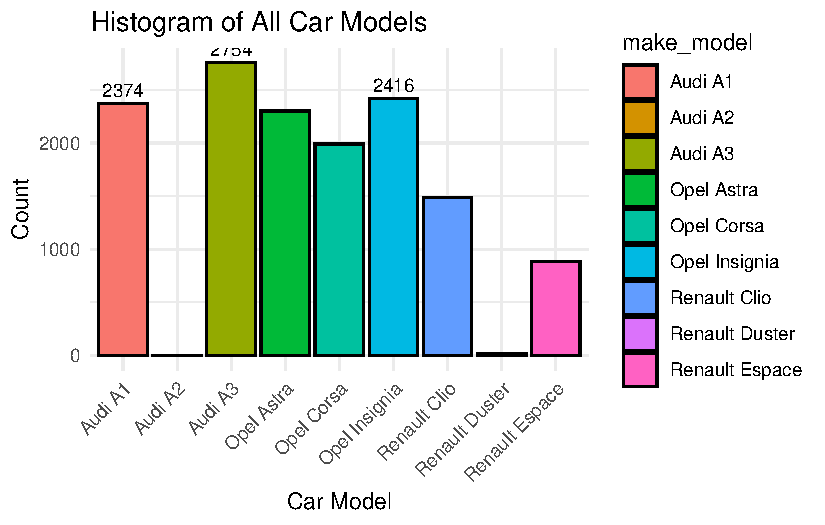
\includegraphics{Sec4_FP_DavidBadalamenti_HsuanYunLiau_RunyiZhang_files/figure-pdf/unnamed-chunk-1-1.pdf}

Choosing larger sample size for these models ensures the results are
statistically reliable and can help better evaluate how variables like
mileage and age impact the prices within and across top models. By
finding the regressions coefficient for both age and mileage we can see
which has a larger impact on the price of the car.

We used a cleaned dataset to get the numerical statistics of what we
wanted to look at directly age, price and mileage.

\begin{Shaded}
\begin{Highlighting}[]
\FunctionTok{library}\NormalTok{(readr)}
\FunctionTok{library}\NormalTok{(dplyr)}
\NormalTok{data }\OtherTok{\textless{}{-}} \FunctionTok{read.csv}\NormalTok{(}\StringTok{"final\_scout\_not\_dummy.csv"}\NormalTok{)}

\FunctionTok{library}\NormalTok{(tidyverse)}

\NormalTok{data }\OtherTok{\textless{}{-}} \FunctionTok{read.csv}\NormalTok{(}\StringTok{"cleaned\_scout\_data.csv"}\NormalTok{)}

\NormalTok{model\_counts }\OtherTok{\textless{}{-}}\NormalTok{ data }\SpecialCharTok{\%\textgreater{}\%} 
  \FunctionTok{group\_by}\NormalTok{(make\_model) }\SpecialCharTok{\%\textgreater{}\%} 
  \FunctionTok{summarise}\NormalTok{(}\AttributeTok{count =} \FunctionTok{n}\NormalTok{()) }\SpecialCharTok{\%\textgreater{}\%} 
  \FunctionTok{arrange}\NormalTok{(}\FunctionTok{desc}\NormalTok{(count))}

\NormalTok{top\_3\_models }\OtherTok{\textless{}{-}} \FunctionTok{head}\NormalTok{(model\_counts, }\DecValTok{3}\NormalTok{)}

\FunctionTok{library}\NormalTok{(ggplot2)}
\FunctionTok{ggplot}\NormalTok{(data, }\FunctionTok{aes}\NormalTok{(}\AttributeTok{x =}\NormalTok{ make\_model, }\AttributeTok{fill =}\NormalTok{ make\_model)) }\SpecialCharTok{+}
  \FunctionTok{geom\_bar}\NormalTok{(}\AttributeTok{color =} \StringTok{"black"}\NormalTok{) }\SpecialCharTok{+}
  \FunctionTok{geom\_text}\NormalTok{(}\AttributeTok{data =}\NormalTok{ top\_3\_models, }\FunctionTok{aes}\NormalTok{(}\AttributeTok{x =}\NormalTok{ make\_model, }\AttributeTok{y =}\NormalTok{ count, }\AttributeTok{label =}\NormalTok{ count), }
            \AttributeTok{vjust =} \SpecialCharTok{{-}}\FloatTok{0.5}\NormalTok{, }\AttributeTok{color =} \StringTok{"black"}\NormalTok{, }\AttributeTok{size =} \DecValTok{3}\NormalTok{) }\SpecialCharTok{+}
  \FunctionTok{labs}\NormalTok{(}
    \AttributeTok{title =} \StringTok{"Histogram of All Car Models"}\NormalTok{,}
    \AttributeTok{x =} \StringTok{"Car Model"}\NormalTok{,}
    \AttributeTok{y =} \StringTok{"Count"}
\NormalTok{  ) }\SpecialCharTok{+}
  \FunctionTok{theme\_minimal}\NormalTok{() }\SpecialCharTok{+}
  \FunctionTok{theme}\NormalTok{(}\AttributeTok{axis.text.x =} \FunctionTok{element\_text}\NormalTok{(}\AttributeTok{angle =} \DecValTok{45}\NormalTok{, }\AttributeTok{hjust =} \DecValTok{1}\NormalTok{))}


\CommentTok{\#Provides key statistics for price, mileage, and age}
\NormalTok{summary\_table }\OtherTok{\textless{}{-}}\NormalTok{ data }\SpecialCharTok{\%\textgreater{}\%}
  \FunctionTok{filter}\NormalTok{(make\_model }\SpecialCharTok{\%in\%} \FunctionTok{c}\NormalTok{(}\StringTok{"Audi A3"}\NormalTok{, }\StringTok{"Opel Insignia"}\NormalTok{, }\StringTok{"Audi A1"}\NormalTok{)) }\SpecialCharTok{\%\textgreater{}\%}
  \FunctionTok{group\_by}\NormalTok{(make\_model) }\SpecialCharTok{\%\textgreater{}\%}
  \FunctionTok{summarise}\NormalTok{(}
    \AttributeTok{Avg\_Price =} \FunctionTok{mean}\NormalTok{(price, }\AttributeTok{na.rm =} \ConstantTok{TRUE}\NormalTok{),}
    \AttributeTok{Median\_Price =} \FunctionTok{median}\NormalTok{(price, }\AttributeTok{na.rm =} \ConstantTok{TRUE}\NormalTok{),}
    \AttributeTok{Min\_Price =} \FunctionTok{min}\NormalTok{(price, }\AttributeTok{na.rm =} \ConstantTok{TRUE}\NormalTok{),}
    \AttributeTok{Max\_Price =} \FunctionTok{max}\NormalTok{(price, }\AttributeTok{na.rm =} \ConstantTok{TRUE}\NormalTok{),}
    \AttributeTok{Avg\_Mileage =} \FunctionTok{mean}\NormalTok{(mileage\_km, }\AttributeTok{na.rm =} \ConstantTok{TRUE}\NormalTok{),}
    \AttributeTok{Median\_Mileage =} \FunctionTok{median}\NormalTok{(mileage\_km, }\AttributeTok{na.rm =} \ConstantTok{TRUE}\NormalTok{),}
    \AttributeTok{Min\_Mileage =} \FunctionTok{min}\NormalTok{(mileage\_km, }\AttributeTok{na.rm =} \ConstantTok{TRUE}\NormalTok{),}
    \AttributeTok{Max\_Mileage =} \FunctionTok{max}\NormalTok{(mileage\_km, }\AttributeTok{na.rm =} \ConstantTok{TRUE}\NormalTok{),}
    \AttributeTok{Avg\_Age =} \FunctionTok{mean}\NormalTok{(age, }\AttributeTok{na.rm =} \ConstantTok{TRUE}\NormalTok{),}
    \AttributeTok{Median\_Age =} \FunctionTok{median}\NormalTok{(age, }\AttributeTok{na.rm =} \ConstantTok{TRUE}\NormalTok{),}
    \AttributeTok{Min\_Age =} \FunctionTok{min}\NormalTok{(age, }\AttributeTok{na.rm =} \ConstantTok{TRUE}\NormalTok{),}
    \AttributeTok{Max\_Age =} \FunctionTok{max}\NormalTok{(age, }\AttributeTok{na.rm =} \ConstantTok{TRUE}\NormalTok{)}
\NormalTok{  )}

\FunctionTok{print}\NormalTok{(summary\_table)}
      
\NormalTok{ audi\_a3\_data }\OtherTok{\textless{}{-}}\NormalTok{ data }\SpecialCharTok{\%\textgreater{}\%} \FunctionTok{filter}\NormalTok{(make\_model }\SpecialCharTok{==} \StringTok{"Audi A3"}\NormalTok{)}

\CommentTok{\# Scatter plot with regression line}
\CommentTok{\#ggplot(audi\_a3\_data, aes(x = age, y = price)) +}
  \CommentTok{\#geom\_point(alpha = 0.6) +}
  \CommentTok{\#geom\_smooth(method = "lm", se = TRUE, color = "red") +}
  \CommentTok{\#labs(}
    \CommentTok{\#title = "Price vs Age for Audi A3",}
    \CommentTok{\#x = "Age (years)",}
    \CommentTok{\#y = "Price (in units)"}
  \CommentTok{\#) +}
  \CommentTok{\#theme\_minimal()}
\CommentTok{\#audi\_age\_model \textless{}{-} lm(price \textasciitilde{} age, data = audi\_a3\_data)}
\CommentTok{\#summary(audi\_age\_model)}


\CommentTok{\# Boxplot}
\FunctionTok{ggplot}\NormalTok{(audi\_a3\_data, }\FunctionTok{aes}\NormalTok{(}\AttributeTok{x =} \FunctionTok{factor}\NormalTok{(age), }\AttributeTok{y =}\NormalTok{ price)) }\SpecialCharTok{+}
  \FunctionTok{geom\_boxplot}\NormalTok{(}\AttributeTok{fill =} \StringTok{"pink"}\NormalTok{) }\SpecialCharTok{+}
  \FunctionTok{labs}\NormalTok{(}
    \AttributeTok{title =} \StringTok{"Boxplot of Price by Age for Audi A3"}\NormalTok{,}
    \AttributeTok{x =} \StringTok{"Age (years)"}\NormalTok{,}
    \AttributeTok{y =} \StringTok{"Price (in units)"}
\NormalTok{  ) }\SpecialCharTok{+}
  \FunctionTok{theme\_minimal}\NormalTok{()}

\NormalTok{opel\_insignia\_data }\OtherTok{\textless{}{-}}\NormalTok{ data }\SpecialCharTok{\%\textgreater{}\%} \FunctionTok{filter}\NormalTok{(make\_model }\SpecialCharTok{==} \StringTok{"Opel Insignia"}\NormalTok{)}

\CommentTok{\# Scatter plot with regression line}
\CommentTok{\# ggplot(opel\_insignia\_data, aes(x = age, y = price)) +}
\CommentTok{\#   geom\_point(alpha = 0.6) +}
\CommentTok{\#   geom\_smooth(method = "lm", se = TRUE, color = "blue") +}
\CommentTok{\#   labs(}
\CommentTok{\#     title = "Price vs Age for Opel Insignia",}
\CommentTok{\#     x = "Age (years)",}
\CommentTok{\#     y = "Price (in units)"}
\CommentTok{\#   ) +}
\CommentTok{\#   theme\_minimal()}
\CommentTok{\# }
\CommentTok{\# opel\_age\_model \textless{}{-} lm(price \textasciitilde{} age, data = opel\_insignia\_data)}
\CommentTok{\# summary(opel\_age\_model)}

\CommentTok{\# Boxplot}
\FunctionTok{ggplot}\NormalTok{(opel\_insignia\_data, }\FunctionTok{aes}\NormalTok{(}\AttributeTok{x =} \FunctionTok{factor}\NormalTok{(age), }\AttributeTok{y =}\NormalTok{ price)) }\SpecialCharTok{+}
  \FunctionTok{geom\_boxplot}\NormalTok{(}\AttributeTok{fill =} \StringTok{"lightblue"}\NormalTok{) }\SpecialCharTok{+}
  \FunctionTok{labs}\NormalTok{(}
    \AttributeTok{title =} \StringTok{"Boxplot of Price by Age for Opel Insignia"}\NormalTok{,}
    \AttributeTok{x =} \StringTok{"Age (years)"}\NormalTok{,}
    \AttributeTok{y =} \StringTok{"Price (in units)"}
\NormalTok{  ) }\SpecialCharTok{+}
  \FunctionTok{theme\_minimal}\NormalTok{()}
\NormalTok{audi\_a1\_data }\OtherTok{\textless{}{-}}\NormalTok{ data }\SpecialCharTok{\%\textgreater{}\%} \FunctionTok{filter}\NormalTok{(make\_model }\SpecialCharTok{==} \StringTok{"Audi A1"}\NormalTok{)}

\CommentTok{\# Scatter plot with regression line}
\CommentTok{\# ggplot(audi\_a1\_data, aes(x = age, y = price)) +}
\CommentTok{\#   geom\_point(alpha = 0.6) +}
\CommentTok{\#   geom\_smooth(method = "lm", se = TRUE, color = "green") +}
\CommentTok{\#   labs(}
\CommentTok{\#     title = "Price vs Age for Audi A1",}
\CommentTok{\#     x = "Age (years)",}
\CommentTok{\#     y = "Price (in units)"}
\CommentTok{\#   ) +}
\CommentTok{\#   theme\_minimal()}
\CommentTok{\# }
\CommentTok{\# audi1\_age\_model \textless{}{-} lm(price \textasciitilde{} age, data = audi\_a1\_data)}
\CommentTok{\# summary(audi1\_age\_model)}

\CommentTok{\# Boxplot for price by age for Audi A1}
\FunctionTok{ggplot}\NormalTok{(audi\_a1\_data, }\FunctionTok{aes}\NormalTok{(}\AttributeTok{x =} \FunctionTok{factor}\NormalTok{(age), }\AttributeTok{y =}\NormalTok{ price)) }\SpecialCharTok{+}
  \FunctionTok{geom\_boxplot}\NormalTok{(}\AttributeTok{fill =} \StringTok{"lightgreen"}\NormalTok{) }\SpecialCharTok{+}
  \FunctionTok{labs}\NormalTok{(}
    \AttributeTok{title =} \StringTok{"Boxplot of Price by Age for Audi A1"}\NormalTok{,}
    \AttributeTok{x =} \StringTok{"Age (years)"}\NormalTok{,}
    \AttributeTok{y =} \StringTok{"Price (in units)"}
\NormalTok{  ) }\SpecialCharTok{+}
  \FunctionTok{theme\_minimal}\NormalTok{()}
      
\NormalTok{ audi\_a3\_data }\OtherTok{\textless{}{-}}\NormalTok{ data }\SpecialCharTok{\%\textgreater{}\%} \FunctionTok{filter}\NormalTok{(make\_model }\SpecialCharTok{==} \StringTok{"Audi A3"}\NormalTok{)}

\CommentTok{\# Scatter plot with regression line}
\FunctionTok{ggplot}\NormalTok{(audi\_a3\_data, }\FunctionTok{aes}\NormalTok{(}\AttributeTok{x =}\NormalTok{ age, }\AttributeTok{y =}\NormalTok{ price)) }\SpecialCharTok{+}
\FunctionTok{geom\_point}\NormalTok{(}\AttributeTok{alpha =} \FloatTok{0.6}\NormalTok{) }\SpecialCharTok{+}
\FunctionTok{geom\_smooth}\NormalTok{(}\AttributeTok{method =} \StringTok{"lm"}\NormalTok{, }\AttributeTok{se =} \ConstantTok{TRUE}\NormalTok{, }\AttributeTok{color =} \StringTok{"red"}\NormalTok{) }\SpecialCharTok{+}
\FunctionTok{labs}\NormalTok{(}
\AttributeTok{title =} \StringTok{"Price vs Age for Audi A3"}\NormalTok{,}
\AttributeTok{x =} \StringTok{"Age (years)"}\NormalTok{,}
\AttributeTok{y =} \StringTok{"Price (in units)"}
\NormalTok{) }\SpecialCharTok{+}
\FunctionTok{theme\_minimal}\NormalTok{()}

\CommentTok{\# audi\_age\_model \textless{}{-} lm(price \textasciitilde{} age, data = audi\_a3\_data)}
\CommentTok{\# summary(audi\_age\_model)}
\CommentTok{\# }

\CommentTok{\# Boxplot}
\CommentTok{\# ggplot(audi\_a3\_data, aes(x = factor(age), y = price)) +}
\CommentTok{\#   geom\_boxplot(fill = "pink") +}
\CommentTok{\#   labs(}
\CommentTok{\#     title = "Boxplot of Price by Age for Audi A3",}
\CommentTok{\#     x = "Age (years)",}
\CommentTok{\#     y = "Price (in units)"}
\CommentTok{\#   ) +}
\CommentTok{\#   theme\_minimal()}

\NormalTok{opel\_insignia\_data }\OtherTok{\textless{}{-}}\NormalTok{ data }\SpecialCharTok{\%\textgreater{}\%} \FunctionTok{filter}\NormalTok{(make\_model }\SpecialCharTok{==} \StringTok{"Opel Insignia"}\NormalTok{)}

\CommentTok{\# Scatter plot with regression line}
\FunctionTok{ggplot}\NormalTok{(opel\_insignia\_data, }\FunctionTok{aes}\NormalTok{(}\AttributeTok{x =}\NormalTok{ age, }\AttributeTok{y =}\NormalTok{ price)) }\SpecialCharTok{+}
  \FunctionTok{geom\_point}\NormalTok{(}\AttributeTok{alpha =} \FloatTok{0.6}\NormalTok{) }\SpecialCharTok{+}
  \FunctionTok{geom\_smooth}\NormalTok{(}\AttributeTok{method =} \StringTok{"lm"}\NormalTok{, }\AttributeTok{se =} \ConstantTok{TRUE}\NormalTok{, }\AttributeTok{color =} \StringTok{"blue"}\NormalTok{) }\SpecialCharTok{+}
  \FunctionTok{labs}\NormalTok{(}
    \AttributeTok{title =} \StringTok{"Price vs Age for Opel Insignia"}\NormalTok{,}
    \AttributeTok{x =} \StringTok{"Age (years)"}\NormalTok{,}
    \AttributeTok{y =} \StringTok{"Price (in units)"}
\NormalTok{  ) }\SpecialCharTok{+}
  \FunctionTok{theme\_minimal}\NormalTok{()}

\CommentTok{\# opel\_age\_model \textless{}{-} lm(price \textasciitilde{} age, data = opel\_insignia\_data)}
\CommentTok{\# summary(opel\_age\_model)}

\CommentTok{\# Boxplot}
\CommentTok{\# ggplot(opel\_insignia\_data, aes(x = factor(age), y = price)) +}
\CommentTok{\#   geom\_boxplot(fill = "lightblue") +}
\CommentTok{\#   labs(}
\CommentTok{\#     title = "Boxplot of Price by Age for Opel Insignia",}
\CommentTok{\#     x = "Age (years)",}
\CommentTok{\#     y = "Price (in units)"}
\CommentTok{\#   ) +}
\CommentTok{\#   theme\_minimal()}
\CommentTok{\# audi\_a1\_data \textless{}{-} data \%\textgreater{}\% filter(make\_model == "Audi A1")}

\CommentTok{\# Scatter plot with regression line}
\FunctionTok{ggplot}\NormalTok{(audi\_a1\_data, }\FunctionTok{aes}\NormalTok{(}\AttributeTok{x =}\NormalTok{ age, }\AttributeTok{y =}\NormalTok{ price)) }\SpecialCharTok{+}
  \FunctionTok{geom\_point}\NormalTok{(}\AttributeTok{alpha =} \FloatTok{0.6}\NormalTok{) }\SpecialCharTok{+}
  \FunctionTok{geom\_smooth}\NormalTok{(}\AttributeTok{method =} \StringTok{"lm"}\NormalTok{, }\AttributeTok{se =} \ConstantTok{TRUE}\NormalTok{, }\AttributeTok{color =} \StringTok{"green"}\NormalTok{) }\SpecialCharTok{+}
  \FunctionTok{labs}\NormalTok{(}
    \AttributeTok{title =} \StringTok{"Price vs Age for Audi A1"}\NormalTok{,}
    \AttributeTok{x =} \StringTok{"Age (years)"}\NormalTok{,}
    \AttributeTok{y =} \StringTok{"Price (in units)"}
\NormalTok{  ) }\SpecialCharTok{+}
  \FunctionTok{theme\_minimal}\NormalTok{()}

\CommentTok{\# audi1\_age\_model \textless{}{-} lm(price \textasciitilde{} age, data = audi\_a1\_data)}
\CommentTok{\# summary(audi1\_age\_model)}

\CommentTok{\# Boxplot for price by age for Audi A1}
\CommentTok{\# ggplot(audi\_a1\_data, aes(x = factor(age), y = price)) +}
\CommentTok{\#   geom\_boxplot(fill = "lightgreen") +}
\CommentTok{\#   labs(}
\CommentTok{\#     title = "Boxplot of Price by Age for Audi A1",}
\CommentTok{\#     x = "Age (years)",}
\CommentTok{\#     y = "Price (in units)"}
\CommentTok{\#   ) +}
\CommentTok{\#   theme\_minimal()}
\CommentTok{\#       }
\CommentTok{\# \#scatter plot}
\CommentTok{\# ggplot(audi\_a3\_data, aes(x = mileage\_km, y = price)) +}
\CommentTok{\#   geom\_point(alpha = 0.6) +}
\CommentTok{\#   geom\_smooth(method = "lm", se = TRUE, color = "red") +}
\CommentTok{\#   scale\_x\_continuous(labels = scales::comma, breaks = seq(0, 300000, by = 50000)) +}
\CommentTok{\#   labs(}
\CommentTok{\#     title = "Price vs Mileage for Audi A3",}
\CommentTok{\#     x = "Mileage (km)",}
\CommentTok{\#     y = "Price (in units)"}
\CommentTok{\#   ) +}
\CommentTok{\#   theme\_minimal()}
\CommentTok{\# }
\CommentTok{\# audi\_mile\_model \textless{}{-} lm(price \textasciitilde{} mileage\_km, data = audi\_a3\_data)}
\CommentTok{\# summary(audi\_mile\_model)}

\CommentTok{\# Boxplot}
\FunctionTok{ggplot}\NormalTok{(audi\_a3\_data, }\FunctionTok{aes}\NormalTok{(}\AttributeTok{x =} \FunctionTok{cut}\NormalTok{(mileage\_km, }\AttributeTok{breaks =} \FunctionTok{c}\NormalTok{(}\DecValTok{0}\NormalTok{, }\DecValTok{50000}\NormalTok{, }\DecValTok{100000}\NormalTok{, }\DecValTok{150000}\NormalTok{, }\DecValTok{200000}\NormalTok{, }\DecValTok{250000}\NormalTok{, }\DecValTok{300000}\NormalTok{),}
                                \AttributeTok{labels =} \FunctionTok{c}\NormalTok{(}\StringTok{"0{-}50k"}\NormalTok{, }\StringTok{"50k{-}100k"}\NormalTok{, }\StringTok{"100k{-}150k"}\NormalTok{, }\StringTok{"150k{-}200k"}\NormalTok{, }\StringTok{"200k{-}250k"}\NormalTok{, }\StringTok{"250k{-}300k"}\NormalTok{)),}
                        \AttributeTok{y =}\NormalTok{ price)) }\SpecialCharTok{+}
  \FunctionTok{geom\_boxplot}\NormalTok{(}\AttributeTok{fill =} \StringTok{"pink"}\NormalTok{) }\SpecialCharTok{+}
  \FunctionTok{labs}\NormalTok{(}
    \AttributeTok{title =} \StringTok{"Boxplot of Price by Mileage for Audi A3"}\NormalTok{,}
    \AttributeTok{x =} \StringTok{"Mileage Range (km)"}\NormalTok{,}
    \AttributeTok{y =} \StringTok{"Price (in units)"}
\NormalTok{  ) }\SpecialCharTok{+}
  \FunctionTok{theme\_minimal}\NormalTok{()}

\CommentTok{\# Boxplot}
\FunctionTok{ggplot}\NormalTok{(opel\_insignia\_data, }\FunctionTok{aes}\NormalTok{(}\AttributeTok{x =} \FunctionTok{cut}\NormalTok{(mileage\_km, }\AttributeTok{breaks =} \FunctionTok{c}\NormalTok{(}\DecValTok{0}\NormalTok{, }\DecValTok{50000}\NormalTok{, }\DecValTok{100000}\NormalTok{, }\DecValTok{150000}\NormalTok{, }\DecValTok{200000}\NormalTok{, }\DecValTok{250000}\NormalTok{, }\DecValTok{300000}\NormalTok{),}
                                     \AttributeTok{labels =} \FunctionTok{c}\NormalTok{(}\StringTok{"0{-}50k"}\NormalTok{, }\StringTok{"50k{-}100k"}\NormalTok{, }\StringTok{"100k{-}150k"}\NormalTok{, }\StringTok{"150k{-}200k"}\NormalTok{, }\StringTok{"200k{-}250k"}\NormalTok{, }\StringTok{"250k{-}300k"}\NormalTok{)),}
                             \AttributeTok{y =}\NormalTok{ price)) }\SpecialCharTok{+}
  \FunctionTok{geom\_boxplot}\NormalTok{(}\AttributeTok{fill =} \StringTok{"lightblue"}\NormalTok{) }\SpecialCharTok{+}
  \FunctionTok{labs}\NormalTok{(}
    \AttributeTok{title =} \StringTok{"Boxplot of Price by Mileage for Opel Insignia"}\NormalTok{,}
    \AttributeTok{x =} \StringTok{"Mileage Range (km)"}\NormalTok{,}
    \AttributeTok{y =} \StringTok{"Price (in units)"}
\NormalTok{  ) }\SpecialCharTok{+}
  \FunctionTok{theme\_minimal}\NormalTok{()}

\CommentTok{\# Boxplot}
\CommentTok{\# This plot shows the distribution of price for each mileage group}
\FunctionTok{ggplot}\NormalTok{(audi\_a1\_data, }\FunctionTok{aes}\NormalTok{(}\AttributeTok{x =} \FunctionTok{cut}\NormalTok{(mileage\_km, }\AttributeTok{breaks =} \FunctionTok{c}\NormalTok{(}\DecValTok{0}\NormalTok{, }\DecValTok{50000}\NormalTok{, }\DecValTok{100000}\NormalTok{, }\DecValTok{150000}\NormalTok{, }\DecValTok{200000}\NormalTok{, }\DecValTok{250000}\NormalTok{, }\DecValTok{300000}\NormalTok{),}
                                \AttributeTok{labels =} \FunctionTok{c}\NormalTok{(}\StringTok{"0{-}50k"}\NormalTok{, }\StringTok{"50k{-}100k"}\NormalTok{, }\StringTok{"100k{-}150k"}\NormalTok{, }\StringTok{"150k{-}200k"}\NormalTok{, }\StringTok{"200k{-}250k"}\NormalTok{, }\StringTok{"250k{-}300k"}\NormalTok{)),}
                        \AttributeTok{y =}\NormalTok{ price)) }\SpecialCharTok{+}
  \FunctionTok{geom\_boxplot}\NormalTok{(}\AttributeTok{fill =} \StringTok{"lightgreen"}\NormalTok{) }\SpecialCharTok{+}
  \FunctionTok{labs}\NormalTok{(}
    \AttributeTok{title =} \StringTok{"Boxplot of Price by Mileage for Audi A1"}\NormalTok{,}
    \AttributeTok{x =} \StringTok{"Mileage Range (km)"}\NormalTok{,}
    \AttributeTok{y =} \StringTok{"Price (in units)"}
\NormalTok{  ) }\SpecialCharTok{+}
  \FunctionTok{theme\_minimal}\NormalTok{()}

\CommentTok{\#Scatter plot}
\FunctionTok{ggplot}\NormalTok{(audi\_a1\_data, }\FunctionTok{aes}\NormalTok{(}\AttributeTok{x =}\NormalTok{ mileage\_km, }\AttributeTok{y =}\NormalTok{ price)) }\SpecialCharTok{+}
  \FunctionTok{geom\_point}\NormalTok{(}\AttributeTok{alpha =} \FloatTok{0.6}\NormalTok{) }\SpecialCharTok{+}
  \FunctionTok{geom\_smooth}\NormalTok{(}\AttributeTok{method =} \StringTok{"lm"}\NormalTok{, }\AttributeTok{se =} \ConstantTok{TRUE}\NormalTok{, }\AttributeTok{color =} \StringTok{"green"}\NormalTok{) }\SpecialCharTok{+}
  \FunctionTok{scale\_x\_continuous}\NormalTok{(}\AttributeTok{labels =}\NormalTok{ scales}\SpecialCharTok{::}\NormalTok{comma, }\AttributeTok{breaks =} \FunctionTok{seq}\NormalTok{(}\DecValTok{0}\NormalTok{, }\DecValTok{300000}\NormalTok{, }\AttributeTok{by =} \DecValTok{50000}\NormalTok{)) }\SpecialCharTok{+}
  \FunctionTok{labs}\NormalTok{(}
    \AttributeTok{title =} \StringTok{"Price vs Mileage for Audi A1"}\NormalTok{,}
    \AttributeTok{x =} \StringTok{"Mileage (km)"}\NormalTok{,}
    \AttributeTok{y =} \StringTok{"Price (in units)"}
\NormalTok{  ) }\SpecialCharTok{+}
  \FunctionTok{theme\_minimal}\NormalTok{()}
\CommentTok{\#Scatter plot}
\FunctionTok{ggplot}\NormalTok{(opel\_insignia\_data, }\FunctionTok{aes}\NormalTok{(}\AttributeTok{x =}\NormalTok{ mileage\_km, }\AttributeTok{y =}\NormalTok{ price)) }\SpecialCharTok{+}
  \FunctionTok{geom\_point}\NormalTok{(}\AttributeTok{alpha =} \FloatTok{0.6}\NormalTok{) }\SpecialCharTok{+}
  \FunctionTok{geom\_smooth}\NormalTok{(}\AttributeTok{method =} \StringTok{"lm"}\NormalTok{, }\AttributeTok{se =} \ConstantTok{TRUE}\NormalTok{, }\AttributeTok{color =} \StringTok{"blue"}\NormalTok{) }\SpecialCharTok{+}
  \FunctionTok{scale\_x\_continuous}\NormalTok{(}\AttributeTok{labels =}\NormalTok{ scales}\SpecialCharTok{::}\NormalTok{comma, }\AttributeTok{breaks =} \FunctionTok{seq}\NormalTok{(}\DecValTok{0}\NormalTok{, }\DecValTok{300000}\NormalTok{, }\AttributeTok{by =} \DecValTok{50000}\NormalTok{)) }\SpecialCharTok{+}
  \FunctionTok{labs}\NormalTok{(}
    \AttributeTok{title =} \StringTok{"Price vs Mileage for Opel Insignia"}\NormalTok{,}
    \AttributeTok{x =} \StringTok{"Mileage (km)"}\NormalTok{,}
    \AttributeTok{y =} \StringTok{"Price (in units)"}
\NormalTok{  ) }\SpecialCharTok{+}
  \FunctionTok{theme\_minimal}\NormalTok{()}

\CommentTok{\#scatter plot}
\FunctionTok{ggplot}\NormalTok{(audi\_a3\_data, }\FunctionTok{aes}\NormalTok{(}\AttributeTok{x =}\NormalTok{ mileage\_km, }\AttributeTok{y =}\NormalTok{ price)) }\SpecialCharTok{+}
  \FunctionTok{geom\_point}\NormalTok{(}\AttributeTok{alpha =} \FloatTok{0.6}\NormalTok{) }\SpecialCharTok{+}
  \FunctionTok{geom\_smooth}\NormalTok{(}\AttributeTok{method =} \StringTok{"lm"}\NormalTok{, }\AttributeTok{se =} \ConstantTok{TRUE}\NormalTok{, }\AttributeTok{color =} \StringTok{"red"}\NormalTok{) }\SpecialCharTok{+}
  \FunctionTok{scale\_x\_continuous}\NormalTok{(}\AttributeTok{labels =}\NormalTok{ scales}\SpecialCharTok{::}\NormalTok{comma, }\AttributeTok{breaks =} \FunctionTok{seq}\NormalTok{(}\DecValTok{0}\NormalTok{, }\DecValTok{300000}\NormalTok{, }\AttributeTok{by =} \DecValTok{50000}\NormalTok{)) }\SpecialCharTok{+}
  \FunctionTok{labs}\NormalTok{(}
    \AttributeTok{title =} \StringTok{"Price vs Mileage for Audi A3"}\NormalTok{,}
    \AttributeTok{x =} \StringTok{"Mileage (km)"}\NormalTok{,}
    \AttributeTok{y =} \StringTok{"Price (in units)"}
\NormalTok{  ) }\SpecialCharTok{+}
  \FunctionTok{theme\_minimal}\NormalTok{()}
\end{Highlighting}
\end{Shaded}

Our initial thoughts were that since the Audi A3 has the highest price
and the lowest price the effect of the mileage and age of that model
would be the largest

\#\#\textbf{Age Models} The following are the graphs of the age vs price
for the three different car models

\begin{Shaded}
\begin{Highlighting}[]
\FunctionTok{library}\NormalTok{(readr)}
\FunctionTok{library}\NormalTok{(dplyr)}
\NormalTok{data }\OtherTok{\textless{}{-}} \FunctionTok{read.csv}\NormalTok{(}\StringTok{"final\_scout\_not\_dummy.csv"}\NormalTok{)}

\FunctionTok{library}\NormalTok{(tidyverse)}

\NormalTok{data }\OtherTok{\textless{}{-}} \FunctionTok{read.csv}\NormalTok{(}\StringTok{"cleaned\_scout\_data.csv"}\NormalTok{)}

\NormalTok{model\_counts }\OtherTok{\textless{}{-}}\NormalTok{ data }\SpecialCharTok{\%\textgreater{}\%} 
  \FunctionTok{group\_by}\NormalTok{(make\_model) }\SpecialCharTok{\%\textgreater{}\%} 
  \FunctionTok{summarise}\NormalTok{(}\AttributeTok{count =} \FunctionTok{n}\NormalTok{()) }\SpecialCharTok{\%\textgreater{}\%} 
  \FunctionTok{arrange}\NormalTok{(}\FunctionTok{desc}\NormalTok{(count))}

\NormalTok{top\_3\_models }\OtherTok{\textless{}{-}} \FunctionTok{head}\NormalTok{(model\_counts, }\DecValTok{3}\NormalTok{)}

\FunctionTok{library}\NormalTok{(ggplot2)}
\FunctionTok{ggplot}\NormalTok{(data, }\FunctionTok{aes}\NormalTok{(}\AttributeTok{x =}\NormalTok{ make\_model, }\AttributeTok{fill =}\NormalTok{ make\_model)) }\SpecialCharTok{+}
  \FunctionTok{geom\_bar}\NormalTok{(}\AttributeTok{color =} \StringTok{"black"}\NormalTok{) }\SpecialCharTok{+}
  \FunctionTok{geom\_text}\NormalTok{(}\AttributeTok{data =}\NormalTok{ top\_3\_models, }\FunctionTok{aes}\NormalTok{(}\AttributeTok{x =}\NormalTok{ make\_model, }\AttributeTok{y =}\NormalTok{ count, }\AttributeTok{label =}\NormalTok{ count), }
            \AttributeTok{vjust =} \SpecialCharTok{{-}}\FloatTok{0.5}\NormalTok{, }\AttributeTok{color =} \StringTok{"black"}\NormalTok{, }\AttributeTok{size =} \DecValTok{3}\NormalTok{) }\SpecialCharTok{+}
  \FunctionTok{labs}\NormalTok{(}
    \AttributeTok{title =} \StringTok{"Histogram of All Car Models"}\NormalTok{,}
    \AttributeTok{x =} \StringTok{"Car Model"}\NormalTok{,}
    \AttributeTok{y =} \StringTok{"Count"}
\NormalTok{  ) }\SpecialCharTok{+}
  \FunctionTok{theme\_minimal}\NormalTok{() }\SpecialCharTok{+}
  \FunctionTok{theme}\NormalTok{(}\AttributeTok{axis.text.x =} \FunctionTok{element\_text}\NormalTok{(}\AttributeTok{angle =} \DecValTok{45}\NormalTok{, }\AttributeTok{hjust =} \DecValTok{1}\NormalTok{))}


\CommentTok{\#Provides key statistics for price, mileage, and age}
\NormalTok{summary\_table }\OtherTok{\textless{}{-}}\NormalTok{ data }\SpecialCharTok{\%\textgreater{}\%}
  \FunctionTok{filter}\NormalTok{(make\_model }\SpecialCharTok{\%in\%} \FunctionTok{c}\NormalTok{(}\StringTok{"Audi A3"}\NormalTok{, }\StringTok{"Opel Insignia"}\NormalTok{, }\StringTok{"Audi A1"}\NormalTok{)) }\SpecialCharTok{\%\textgreater{}\%}
  \FunctionTok{group\_by}\NormalTok{(make\_model) }\SpecialCharTok{\%\textgreater{}\%}
  \FunctionTok{summarise}\NormalTok{(}
    \AttributeTok{Avg\_Price =} \FunctionTok{mean}\NormalTok{(price, }\AttributeTok{na.rm =} \ConstantTok{TRUE}\NormalTok{),}
    \AttributeTok{Median\_Price =} \FunctionTok{median}\NormalTok{(price, }\AttributeTok{na.rm =} \ConstantTok{TRUE}\NormalTok{),}
    \AttributeTok{Min\_Price =} \FunctionTok{min}\NormalTok{(price, }\AttributeTok{na.rm =} \ConstantTok{TRUE}\NormalTok{),}
    \AttributeTok{Max\_Price =} \FunctionTok{max}\NormalTok{(price, }\AttributeTok{na.rm =} \ConstantTok{TRUE}\NormalTok{),}
    \AttributeTok{Avg\_Mileage =} \FunctionTok{mean}\NormalTok{(mileage\_km, }\AttributeTok{na.rm =} \ConstantTok{TRUE}\NormalTok{),}
    \AttributeTok{Median\_Mileage =} \FunctionTok{median}\NormalTok{(mileage\_km, }\AttributeTok{na.rm =} \ConstantTok{TRUE}\NormalTok{),}
    \AttributeTok{Min\_Mileage =} \FunctionTok{min}\NormalTok{(mileage\_km, }\AttributeTok{na.rm =} \ConstantTok{TRUE}\NormalTok{),}
    \AttributeTok{Max\_Mileage =} \FunctionTok{max}\NormalTok{(mileage\_km, }\AttributeTok{na.rm =} \ConstantTok{TRUE}\NormalTok{),}
    \AttributeTok{Avg\_Age =} \FunctionTok{mean}\NormalTok{(age, }\AttributeTok{na.rm =} \ConstantTok{TRUE}\NormalTok{),}
    \AttributeTok{Median\_Age =} \FunctionTok{median}\NormalTok{(age, }\AttributeTok{na.rm =} \ConstantTok{TRUE}\NormalTok{),}
    \AttributeTok{Min\_Age =} \FunctionTok{min}\NormalTok{(age, }\AttributeTok{na.rm =} \ConstantTok{TRUE}\NormalTok{),}
    \AttributeTok{Max\_Age =} \FunctionTok{max}\NormalTok{(age, }\AttributeTok{na.rm =} \ConstantTok{TRUE}\NormalTok{)}
\NormalTok{  )}

\FunctionTok{print}\NormalTok{(summary\_table)}
      
\NormalTok{ audi\_a3\_data }\OtherTok{\textless{}{-}}\NormalTok{ data }\SpecialCharTok{\%\textgreater{}\%} \FunctionTok{filter}\NormalTok{(make\_model }\SpecialCharTok{==} \StringTok{"Audi A3"}\NormalTok{)}

\CommentTok{\# Scatter plot with regression line}
\CommentTok{\#ggplot(audi\_a3\_data, aes(x = age, y = price)) +}
  \CommentTok{\#geom\_point(alpha = 0.6) +}
  \CommentTok{\#geom\_smooth(method = "lm", se = TRUE, color = "red") +}
  \CommentTok{\#labs(}
    \CommentTok{\#title = "Price vs Age for Audi A3",}
    \CommentTok{\#x = "Age (years)",}
    \CommentTok{\#y = "Price (in units)"}
  \CommentTok{\#) +}
  \CommentTok{\#theme\_minimal()}
\CommentTok{\#audi\_age\_model \textless{}{-} lm(price \textasciitilde{} age, data = audi\_a3\_data)}
\CommentTok{\#summary(audi\_age\_model)}


\CommentTok{\# Boxplot}
\FunctionTok{ggplot}\NormalTok{(audi\_a3\_data, }\FunctionTok{aes}\NormalTok{(}\AttributeTok{x =} \FunctionTok{factor}\NormalTok{(age), }\AttributeTok{y =}\NormalTok{ price)) }\SpecialCharTok{+}
  \FunctionTok{geom\_boxplot}\NormalTok{(}\AttributeTok{fill =} \StringTok{"pink"}\NormalTok{) }\SpecialCharTok{+}
  \FunctionTok{labs}\NormalTok{(}
    \AttributeTok{title =} \StringTok{"Boxplot of Price by Age for Audi A3"}\NormalTok{,}
    \AttributeTok{x =} \StringTok{"Age (years)"}\NormalTok{,}
    \AttributeTok{y =} \StringTok{"Price (in units)"}
\NormalTok{  ) }\SpecialCharTok{+}
  \FunctionTok{theme\_minimal}\NormalTok{()}

\NormalTok{opel\_insignia\_data }\OtherTok{\textless{}{-}}\NormalTok{ data }\SpecialCharTok{\%\textgreater{}\%} \FunctionTok{filter}\NormalTok{(make\_model }\SpecialCharTok{==} \StringTok{"Opel Insignia"}\NormalTok{)}

\CommentTok{\# Scatter plot with regression line}
\CommentTok{\# ggplot(opel\_insignia\_data, aes(x = age, y = price)) +}
\CommentTok{\#   geom\_point(alpha = 0.6) +}
\CommentTok{\#   geom\_smooth(method = "lm", se = TRUE, color = "blue") +}
\CommentTok{\#   labs(}
\CommentTok{\#     title = "Price vs Age for Opel Insignia",}
\CommentTok{\#     x = "Age (years)",}
\CommentTok{\#     y = "Price (in units)"}
\CommentTok{\#   ) +}
\CommentTok{\#   theme\_minimal()}
\CommentTok{\# }
\CommentTok{\# opel\_age\_model \textless{}{-} lm(price \textasciitilde{} age, data = opel\_insignia\_data)}
\CommentTok{\# summary(opel\_age\_model)}

\CommentTok{\# Boxplot}
\FunctionTok{ggplot}\NormalTok{(opel\_insignia\_data, }\FunctionTok{aes}\NormalTok{(}\AttributeTok{x =} \FunctionTok{factor}\NormalTok{(age), }\AttributeTok{y =}\NormalTok{ price)) }\SpecialCharTok{+}
  \FunctionTok{geom\_boxplot}\NormalTok{(}\AttributeTok{fill =} \StringTok{"lightblue"}\NormalTok{) }\SpecialCharTok{+}
  \FunctionTok{labs}\NormalTok{(}
    \AttributeTok{title =} \StringTok{"Boxplot of Price by Age for Opel Insignia"}\NormalTok{,}
    \AttributeTok{x =} \StringTok{"Age (years)"}\NormalTok{,}
    \AttributeTok{y =} \StringTok{"Price (in units)"}
\NormalTok{  ) }\SpecialCharTok{+}
  \FunctionTok{theme\_minimal}\NormalTok{()}
\NormalTok{audi\_a1\_data }\OtherTok{\textless{}{-}}\NormalTok{ data }\SpecialCharTok{\%\textgreater{}\%} \FunctionTok{filter}\NormalTok{(make\_model }\SpecialCharTok{==} \StringTok{"Audi A1"}\NormalTok{)}

\CommentTok{\# Scatter plot with regression line}
\CommentTok{\# ggplot(audi\_a1\_data, aes(x = age, y = price)) +}
\CommentTok{\#   geom\_point(alpha = 0.6) +}
\CommentTok{\#   geom\_smooth(method = "lm", se = TRUE, color = "green") +}
\CommentTok{\#   labs(}
\CommentTok{\#     title = "Price vs Age for Audi A1",}
\CommentTok{\#     x = "Age (years)",}
\CommentTok{\#     y = "Price (in units)"}
\CommentTok{\#   ) +}
\CommentTok{\#   theme\_minimal()}
\CommentTok{\# }
\CommentTok{\# audi1\_age\_model \textless{}{-} lm(price \textasciitilde{} age, data = audi\_a1\_data)}
\CommentTok{\# summary(audi1\_age\_model)}

\CommentTok{\# Boxplot for price by age for Audi A1}
\FunctionTok{ggplot}\NormalTok{(audi\_a1\_data, }\FunctionTok{aes}\NormalTok{(}\AttributeTok{x =} \FunctionTok{factor}\NormalTok{(age), }\AttributeTok{y =}\NormalTok{ price)) }\SpecialCharTok{+}
  \FunctionTok{geom\_boxplot}\NormalTok{(}\AttributeTok{fill =} \StringTok{"lightgreen"}\NormalTok{) }\SpecialCharTok{+}
  \FunctionTok{labs}\NormalTok{(}
    \AttributeTok{title =} \StringTok{"Boxplot of Price by Age for Audi A1"}\NormalTok{,}
    \AttributeTok{x =} \StringTok{"Age (years)"}\NormalTok{,}
    \AttributeTok{y =} \StringTok{"Price (in units)"}
\NormalTok{  ) }\SpecialCharTok{+}
  \FunctionTok{theme\_minimal}\NormalTok{()}
      
\NormalTok{ audi\_a3\_data }\OtherTok{\textless{}{-}}\NormalTok{ data }\SpecialCharTok{\%\textgreater{}\%} \FunctionTok{filter}\NormalTok{(make\_model }\SpecialCharTok{==} \StringTok{"Audi A3"}\NormalTok{)}

\CommentTok{\# Scatter plot with regression line}
\FunctionTok{ggplot}\NormalTok{(audi\_a3\_data, }\FunctionTok{aes}\NormalTok{(}\AttributeTok{x =}\NormalTok{ age, }\AttributeTok{y =}\NormalTok{ price)) }\SpecialCharTok{+}
\FunctionTok{geom\_point}\NormalTok{(}\AttributeTok{alpha =} \FloatTok{0.6}\NormalTok{) }\SpecialCharTok{+}
\FunctionTok{geom\_smooth}\NormalTok{(}\AttributeTok{method =} \StringTok{"lm"}\NormalTok{, }\AttributeTok{se =} \ConstantTok{TRUE}\NormalTok{, }\AttributeTok{color =} \StringTok{"red"}\NormalTok{) }\SpecialCharTok{+}
\FunctionTok{labs}\NormalTok{(}
\AttributeTok{title =} \StringTok{"Price vs Age for Audi A3"}\NormalTok{,}
\AttributeTok{x =} \StringTok{"Age (years)"}\NormalTok{,}
\AttributeTok{y =} \StringTok{"Price (in units)"}
\NormalTok{) }\SpecialCharTok{+}
\FunctionTok{theme\_minimal}\NormalTok{()}

\CommentTok{\# audi\_age\_model \textless{}{-} lm(price \textasciitilde{} age, data = audi\_a3\_data)}
\CommentTok{\# summary(audi\_age\_model)}
\CommentTok{\# }

\CommentTok{\# Boxplot}
\CommentTok{\# ggplot(audi\_a3\_data, aes(x = factor(age), y = price)) +}
\CommentTok{\#   geom\_boxplot(fill = "pink") +}
\CommentTok{\#   labs(}
\CommentTok{\#     title = "Boxplot of Price by Age for Audi A3",}
\CommentTok{\#     x = "Age (years)",}
\CommentTok{\#     y = "Price (in units)"}
\CommentTok{\#   ) +}
\CommentTok{\#   theme\_minimal()}

\NormalTok{opel\_insignia\_data }\OtherTok{\textless{}{-}}\NormalTok{ data }\SpecialCharTok{\%\textgreater{}\%} \FunctionTok{filter}\NormalTok{(make\_model }\SpecialCharTok{==} \StringTok{"Opel Insignia"}\NormalTok{)}

\CommentTok{\# Scatter plot with regression line}
\FunctionTok{ggplot}\NormalTok{(opel\_insignia\_data, }\FunctionTok{aes}\NormalTok{(}\AttributeTok{x =}\NormalTok{ age, }\AttributeTok{y =}\NormalTok{ price)) }\SpecialCharTok{+}
  \FunctionTok{geom\_point}\NormalTok{(}\AttributeTok{alpha =} \FloatTok{0.6}\NormalTok{) }\SpecialCharTok{+}
  \FunctionTok{geom\_smooth}\NormalTok{(}\AttributeTok{method =} \StringTok{"lm"}\NormalTok{, }\AttributeTok{se =} \ConstantTok{TRUE}\NormalTok{, }\AttributeTok{color =} \StringTok{"blue"}\NormalTok{) }\SpecialCharTok{+}
  \FunctionTok{labs}\NormalTok{(}
    \AttributeTok{title =} \StringTok{"Price vs Age for Opel Insignia"}\NormalTok{,}
    \AttributeTok{x =} \StringTok{"Age (years)"}\NormalTok{,}
    \AttributeTok{y =} \StringTok{"Price (in units)"}
\NormalTok{  ) }\SpecialCharTok{+}
  \FunctionTok{theme\_minimal}\NormalTok{()}

\CommentTok{\# opel\_age\_model \textless{}{-} lm(price \textasciitilde{} age, data = opel\_insignia\_data)}
\CommentTok{\# summary(opel\_age\_model)}

\CommentTok{\# Boxplot}
\CommentTok{\# ggplot(opel\_insignia\_data, aes(x = factor(age), y = price)) +}
\CommentTok{\#   geom\_boxplot(fill = "lightblue") +}
\CommentTok{\#   labs(}
\CommentTok{\#     title = "Boxplot of Price by Age for Opel Insignia",}
\CommentTok{\#     x = "Age (years)",}
\CommentTok{\#     y = "Price (in units)"}
\CommentTok{\#   ) +}
\CommentTok{\#   theme\_minimal()}
\CommentTok{\# audi\_a1\_data \textless{}{-} data \%\textgreater{}\% filter(make\_model == "Audi A1")}

\CommentTok{\# Scatter plot with regression line}
\FunctionTok{ggplot}\NormalTok{(audi\_a1\_data, }\FunctionTok{aes}\NormalTok{(}\AttributeTok{x =}\NormalTok{ age, }\AttributeTok{y =}\NormalTok{ price)) }\SpecialCharTok{+}
  \FunctionTok{geom\_point}\NormalTok{(}\AttributeTok{alpha =} \FloatTok{0.6}\NormalTok{) }\SpecialCharTok{+}
  \FunctionTok{geom\_smooth}\NormalTok{(}\AttributeTok{method =} \StringTok{"lm"}\NormalTok{, }\AttributeTok{se =} \ConstantTok{TRUE}\NormalTok{, }\AttributeTok{color =} \StringTok{"green"}\NormalTok{) }\SpecialCharTok{+}
  \FunctionTok{labs}\NormalTok{(}
    \AttributeTok{title =} \StringTok{"Price vs Age for Audi A1"}\NormalTok{,}
    \AttributeTok{x =} \StringTok{"Age (years)"}\NormalTok{,}
    \AttributeTok{y =} \StringTok{"Price (in units)"}
\NormalTok{  ) }\SpecialCharTok{+}
  \FunctionTok{theme\_minimal}\NormalTok{()}

\CommentTok{\# audi1\_age\_model \textless{}{-} lm(price \textasciitilde{} age, data = audi\_a1\_data)}
\CommentTok{\# summary(audi1\_age\_model)}

\CommentTok{\# Boxplot for price by age for Audi A1}
\CommentTok{\# ggplot(audi\_a1\_data, aes(x = factor(age), y = price)) +}
\CommentTok{\#   geom\_boxplot(fill = "lightgreen") +}
\CommentTok{\#   labs(}
\CommentTok{\#     title = "Boxplot of Price by Age for Audi A1",}
\CommentTok{\#     x = "Age (years)",}
\CommentTok{\#     y = "Price (in units)"}
\CommentTok{\#   ) +}
\CommentTok{\#   theme\_minimal()}
\CommentTok{\#       }
\CommentTok{\# \#scatter plot}
\CommentTok{\# ggplot(audi\_a3\_data, aes(x = mileage\_km, y = price)) +}
\CommentTok{\#   geom\_point(alpha = 0.6) +}
\CommentTok{\#   geom\_smooth(method = "lm", se = TRUE, color = "red") +}
\CommentTok{\#   scale\_x\_continuous(labels = scales::comma, breaks = seq(0, 300000, by = 50000)) +}
\CommentTok{\#   labs(}
\CommentTok{\#     title = "Price vs Mileage for Audi A3",}
\CommentTok{\#     x = "Mileage (km)",}
\CommentTok{\#     y = "Price (in units)"}
\CommentTok{\#   ) +}
\CommentTok{\#   theme\_minimal()}
\CommentTok{\# }
\CommentTok{\# audi\_mile\_model \textless{}{-} lm(price \textasciitilde{} mileage\_km, data = audi\_a3\_data)}
\CommentTok{\# summary(audi\_mile\_model)}

\CommentTok{\# Boxplot}
\FunctionTok{ggplot}\NormalTok{(audi\_a3\_data, }\FunctionTok{aes}\NormalTok{(}\AttributeTok{x =} \FunctionTok{cut}\NormalTok{(mileage\_km, }\AttributeTok{breaks =} \FunctionTok{c}\NormalTok{(}\DecValTok{0}\NormalTok{, }\DecValTok{50000}\NormalTok{, }\DecValTok{100000}\NormalTok{, }\DecValTok{150000}\NormalTok{, }\DecValTok{200000}\NormalTok{, }\DecValTok{250000}\NormalTok{, }\DecValTok{300000}\NormalTok{),}
                                \AttributeTok{labels =} \FunctionTok{c}\NormalTok{(}\StringTok{"0{-}50k"}\NormalTok{, }\StringTok{"50k{-}100k"}\NormalTok{, }\StringTok{"100k{-}150k"}\NormalTok{, }\StringTok{"150k{-}200k"}\NormalTok{, }\StringTok{"200k{-}250k"}\NormalTok{, }\StringTok{"250k{-}300k"}\NormalTok{)),}
                        \AttributeTok{y =}\NormalTok{ price)) }\SpecialCharTok{+}
  \FunctionTok{geom\_boxplot}\NormalTok{(}\AttributeTok{fill =} \StringTok{"pink"}\NormalTok{) }\SpecialCharTok{+}
  \FunctionTok{labs}\NormalTok{(}
    \AttributeTok{title =} \StringTok{"Boxplot of Price by Mileage for Audi A3"}\NormalTok{,}
    \AttributeTok{x =} \StringTok{"Mileage Range (km)"}\NormalTok{,}
    \AttributeTok{y =} \StringTok{"Price (in units)"}
\NormalTok{  ) }\SpecialCharTok{+}
  \FunctionTok{theme\_minimal}\NormalTok{()}

\CommentTok{\# Boxplot}
\FunctionTok{ggplot}\NormalTok{(opel\_insignia\_data, }\FunctionTok{aes}\NormalTok{(}\AttributeTok{x =} \FunctionTok{cut}\NormalTok{(mileage\_km, }\AttributeTok{breaks =} \FunctionTok{c}\NormalTok{(}\DecValTok{0}\NormalTok{, }\DecValTok{50000}\NormalTok{, }\DecValTok{100000}\NormalTok{, }\DecValTok{150000}\NormalTok{, }\DecValTok{200000}\NormalTok{, }\DecValTok{250000}\NormalTok{, }\DecValTok{300000}\NormalTok{),}
                                     \AttributeTok{labels =} \FunctionTok{c}\NormalTok{(}\StringTok{"0{-}50k"}\NormalTok{, }\StringTok{"50k{-}100k"}\NormalTok{, }\StringTok{"100k{-}150k"}\NormalTok{, }\StringTok{"150k{-}200k"}\NormalTok{, }\StringTok{"200k{-}250k"}\NormalTok{, }\StringTok{"250k{-}300k"}\NormalTok{)),}
                             \AttributeTok{y =}\NormalTok{ price)) }\SpecialCharTok{+}
  \FunctionTok{geom\_boxplot}\NormalTok{(}\AttributeTok{fill =} \StringTok{"lightblue"}\NormalTok{) }\SpecialCharTok{+}
  \FunctionTok{labs}\NormalTok{(}
    \AttributeTok{title =} \StringTok{"Boxplot of Price by Mileage for Opel Insignia"}\NormalTok{,}
    \AttributeTok{x =} \StringTok{"Mileage Range (km)"}\NormalTok{,}
    \AttributeTok{y =} \StringTok{"Price (in units)"}
\NormalTok{  ) }\SpecialCharTok{+}
  \FunctionTok{theme\_minimal}\NormalTok{()}

\CommentTok{\# Boxplot}
\CommentTok{\# This plot shows the distribution of price for each mileage group}
\FunctionTok{ggplot}\NormalTok{(audi\_a1\_data, }\FunctionTok{aes}\NormalTok{(}\AttributeTok{x =} \FunctionTok{cut}\NormalTok{(mileage\_km, }\AttributeTok{breaks =} \FunctionTok{c}\NormalTok{(}\DecValTok{0}\NormalTok{, }\DecValTok{50000}\NormalTok{, }\DecValTok{100000}\NormalTok{, }\DecValTok{150000}\NormalTok{, }\DecValTok{200000}\NormalTok{, }\DecValTok{250000}\NormalTok{, }\DecValTok{300000}\NormalTok{),}
                                \AttributeTok{labels =} \FunctionTok{c}\NormalTok{(}\StringTok{"0{-}50k"}\NormalTok{, }\StringTok{"50k{-}100k"}\NormalTok{, }\StringTok{"100k{-}150k"}\NormalTok{, }\StringTok{"150k{-}200k"}\NormalTok{, }\StringTok{"200k{-}250k"}\NormalTok{, }\StringTok{"250k{-}300k"}\NormalTok{)),}
                        \AttributeTok{y =}\NormalTok{ price)) }\SpecialCharTok{+}
  \FunctionTok{geom\_boxplot}\NormalTok{(}\AttributeTok{fill =} \StringTok{"lightgreen"}\NormalTok{) }\SpecialCharTok{+}
  \FunctionTok{labs}\NormalTok{(}
    \AttributeTok{title =} \StringTok{"Boxplot of Price by Mileage for Audi A1"}\NormalTok{,}
    \AttributeTok{x =} \StringTok{"Mileage Range (km)"}\NormalTok{,}
    \AttributeTok{y =} \StringTok{"Price (in units)"}
\NormalTok{  ) }\SpecialCharTok{+}
  \FunctionTok{theme\_minimal}\NormalTok{()}

\CommentTok{\#Scatter plot}
\FunctionTok{ggplot}\NormalTok{(audi\_a1\_data, }\FunctionTok{aes}\NormalTok{(}\AttributeTok{x =}\NormalTok{ mileage\_km, }\AttributeTok{y =}\NormalTok{ price)) }\SpecialCharTok{+}
  \FunctionTok{geom\_point}\NormalTok{(}\AttributeTok{alpha =} \FloatTok{0.6}\NormalTok{) }\SpecialCharTok{+}
  \FunctionTok{geom\_smooth}\NormalTok{(}\AttributeTok{method =} \StringTok{"lm"}\NormalTok{, }\AttributeTok{se =} \ConstantTok{TRUE}\NormalTok{, }\AttributeTok{color =} \StringTok{"green"}\NormalTok{) }\SpecialCharTok{+}
  \FunctionTok{scale\_x\_continuous}\NormalTok{(}\AttributeTok{labels =}\NormalTok{ scales}\SpecialCharTok{::}\NormalTok{comma, }\AttributeTok{breaks =} \FunctionTok{seq}\NormalTok{(}\DecValTok{0}\NormalTok{, }\DecValTok{300000}\NormalTok{, }\AttributeTok{by =} \DecValTok{50000}\NormalTok{)) }\SpecialCharTok{+}
  \FunctionTok{labs}\NormalTok{(}
    \AttributeTok{title =} \StringTok{"Price vs Mileage for Audi A1"}\NormalTok{,}
    \AttributeTok{x =} \StringTok{"Mileage (km)"}\NormalTok{,}
    \AttributeTok{y =} \StringTok{"Price (in units)"}
\NormalTok{  ) }\SpecialCharTok{+}
  \FunctionTok{theme\_minimal}\NormalTok{()}
\CommentTok{\#Scatter plot}
\FunctionTok{ggplot}\NormalTok{(opel\_insignia\_data, }\FunctionTok{aes}\NormalTok{(}\AttributeTok{x =}\NormalTok{ mileage\_km, }\AttributeTok{y =}\NormalTok{ price)) }\SpecialCharTok{+}
  \FunctionTok{geom\_point}\NormalTok{(}\AttributeTok{alpha =} \FloatTok{0.6}\NormalTok{) }\SpecialCharTok{+}
  \FunctionTok{geom\_smooth}\NormalTok{(}\AttributeTok{method =} \StringTok{"lm"}\NormalTok{, }\AttributeTok{se =} \ConstantTok{TRUE}\NormalTok{, }\AttributeTok{color =} \StringTok{"blue"}\NormalTok{) }\SpecialCharTok{+}
  \FunctionTok{scale\_x\_continuous}\NormalTok{(}\AttributeTok{labels =}\NormalTok{ scales}\SpecialCharTok{::}\NormalTok{comma, }\AttributeTok{breaks =} \FunctionTok{seq}\NormalTok{(}\DecValTok{0}\NormalTok{, }\DecValTok{300000}\NormalTok{, }\AttributeTok{by =} \DecValTok{50000}\NormalTok{)) }\SpecialCharTok{+}
  \FunctionTok{labs}\NormalTok{(}
    \AttributeTok{title =} \StringTok{"Price vs Mileage for Opel Insignia"}\NormalTok{,}
    \AttributeTok{x =} \StringTok{"Mileage (km)"}\NormalTok{,}
    \AttributeTok{y =} \StringTok{"Price (in units)"}
\NormalTok{  ) }\SpecialCharTok{+}
  \FunctionTok{theme\_minimal}\NormalTok{()}

\CommentTok{\#scatter plot}
\FunctionTok{ggplot}\NormalTok{(audi\_a3\_data, }\FunctionTok{aes}\NormalTok{(}\AttributeTok{x =}\NormalTok{ mileage\_km, }\AttributeTok{y =}\NormalTok{ price)) }\SpecialCharTok{+}
  \FunctionTok{geom\_point}\NormalTok{(}\AttributeTok{alpha =} \FloatTok{0.6}\NormalTok{) }\SpecialCharTok{+}
  \FunctionTok{geom\_smooth}\NormalTok{(}\AttributeTok{method =} \StringTok{"lm"}\NormalTok{, }\AttributeTok{se =} \ConstantTok{TRUE}\NormalTok{, }\AttributeTok{color =} \StringTok{"red"}\NormalTok{) }\SpecialCharTok{+}
  \FunctionTok{scale\_x\_continuous}\NormalTok{(}\AttributeTok{labels =}\NormalTok{ scales}\SpecialCharTok{::}\NormalTok{comma, }\AttributeTok{breaks =} \FunctionTok{seq}\NormalTok{(}\DecValTok{0}\NormalTok{, }\DecValTok{300000}\NormalTok{, }\AttributeTok{by =} \DecValTok{50000}\NormalTok{)) }\SpecialCharTok{+}
  \FunctionTok{labs}\NormalTok{(}
    \AttributeTok{title =} \StringTok{"Price vs Mileage for Audi A3"}\NormalTok{,}
    \AttributeTok{x =} \StringTok{"Mileage (km)"}\NormalTok{,}
    \AttributeTok{y =} \StringTok{"Price (in units)"}
\NormalTok{  ) }\SpecialCharTok{+}
  \FunctionTok{theme\_minimal}\NormalTok{()}
\end{Highlighting}
\end{Shaded}

After Visualizing the data with a box plot we create a scatter plot with
a regression line to see the change in price by age

\begin{Shaded}
\begin{Highlighting}[]
\FunctionTok{library}\NormalTok{(readr)}
\FunctionTok{library}\NormalTok{(dplyr)}
\NormalTok{data }\OtherTok{\textless{}{-}} \FunctionTok{read.csv}\NormalTok{(}\StringTok{"final\_scout\_not\_dummy.csv"}\NormalTok{)}

\FunctionTok{library}\NormalTok{(tidyverse)}

\NormalTok{data }\OtherTok{\textless{}{-}} \FunctionTok{read.csv}\NormalTok{(}\StringTok{"cleaned\_scout\_data.csv"}\NormalTok{)}

\NormalTok{model\_counts }\OtherTok{\textless{}{-}}\NormalTok{ data }\SpecialCharTok{\%\textgreater{}\%} 
  \FunctionTok{group\_by}\NormalTok{(make\_model) }\SpecialCharTok{\%\textgreater{}\%} 
  \FunctionTok{summarise}\NormalTok{(}\AttributeTok{count =} \FunctionTok{n}\NormalTok{()) }\SpecialCharTok{\%\textgreater{}\%} 
  \FunctionTok{arrange}\NormalTok{(}\FunctionTok{desc}\NormalTok{(count))}

\NormalTok{top\_3\_models }\OtherTok{\textless{}{-}} \FunctionTok{head}\NormalTok{(model\_counts, }\DecValTok{3}\NormalTok{)}

\FunctionTok{library}\NormalTok{(ggplot2)}
\FunctionTok{ggplot}\NormalTok{(data, }\FunctionTok{aes}\NormalTok{(}\AttributeTok{x =}\NormalTok{ make\_model, }\AttributeTok{fill =}\NormalTok{ make\_model)) }\SpecialCharTok{+}
  \FunctionTok{geom\_bar}\NormalTok{(}\AttributeTok{color =} \StringTok{"black"}\NormalTok{) }\SpecialCharTok{+}
  \FunctionTok{geom\_text}\NormalTok{(}\AttributeTok{data =}\NormalTok{ top\_3\_models, }\FunctionTok{aes}\NormalTok{(}\AttributeTok{x =}\NormalTok{ make\_model, }\AttributeTok{y =}\NormalTok{ count, }\AttributeTok{label =}\NormalTok{ count), }
            \AttributeTok{vjust =} \SpecialCharTok{{-}}\FloatTok{0.5}\NormalTok{, }\AttributeTok{color =} \StringTok{"black"}\NormalTok{, }\AttributeTok{size =} \DecValTok{3}\NormalTok{) }\SpecialCharTok{+}
  \FunctionTok{labs}\NormalTok{(}
    \AttributeTok{title =} \StringTok{"Histogram of All Car Models"}\NormalTok{,}
    \AttributeTok{x =} \StringTok{"Car Model"}\NormalTok{,}
    \AttributeTok{y =} \StringTok{"Count"}
\NormalTok{  ) }\SpecialCharTok{+}
  \FunctionTok{theme\_minimal}\NormalTok{() }\SpecialCharTok{+}
  \FunctionTok{theme}\NormalTok{(}\AttributeTok{axis.text.x =} \FunctionTok{element\_text}\NormalTok{(}\AttributeTok{angle =} \DecValTok{45}\NormalTok{, }\AttributeTok{hjust =} \DecValTok{1}\NormalTok{))}


\CommentTok{\#Provides key statistics for price, mileage, and age}
\NormalTok{summary\_table }\OtherTok{\textless{}{-}}\NormalTok{ data }\SpecialCharTok{\%\textgreater{}\%}
  \FunctionTok{filter}\NormalTok{(make\_model }\SpecialCharTok{\%in\%} \FunctionTok{c}\NormalTok{(}\StringTok{"Audi A3"}\NormalTok{, }\StringTok{"Opel Insignia"}\NormalTok{, }\StringTok{"Audi A1"}\NormalTok{)) }\SpecialCharTok{\%\textgreater{}\%}
  \FunctionTok{group\_by}\NormalTok{(make\_model) }\SpecialCharTok{\%\textgreater{}\%}
  \FunctionTok{summarise}\NormalTok{(}
    \AttributeTok{Avg\_Price =} \FunctionTok{mean}\NormalTok{(price, }\AttributeTok{na.rm =} \ConstantTok{TRUE}\NormalTok{),}
    \AttributeTok{Median\_Price =} \FunctionTok{median}\NormalTok{(price, }\AttributeTok{na.rm =} \ConstantTok{TRUE}\NormalTok{),}
    \AttributeTok{Min\_Price =} \FunctionTok{min}\NormalTok{(price, }\AttributeTok{na.rm =} \ConstantTok{TRUE}\NormalTok{),}
    \AttributeTok{Max\_Price =} \FunctionTok{max}\NormalTok{(price, }\AttributeTok{na.rm =} \ConstantTok{TRUE}\NormalTok{),}
    \AttributeTok{Avg\_Mileage =} \FunctionTok{mean}\NormalTok{(mileage\_km, }\AttributeTok{na.rm =} \ConstantTok{TRUE}\NormalTok{),}
    \AttributeTok{Median\_Mileage =} \FunctionTok{median}\NormalTok{(mileage\_km, }\AttributeTok{na.rm =} \ConstantTok{TRUE}\NormalTok{),}
    \AttributeTok{Min\_Mileage =} \FunctionTok{min}\NormalTok{(mileage\_km, }\AttributeTok{na.rm =} \ConstantTok{TRUE}\NormalTok{),}
    \AttributeTok{Max\_Mileage =} \FunctionTok{max}\NormalTok{(mileage\_km, }\AttributeTok{na.rm =} \ConstantTok{TRUE}\NormalTok{),}
    \AttributeTok{Avg\_Age =} \FunctionTok{mean}\NormalTok{(age, }\AttributeTok{na.rm =} \ConstantTok{TRUE}\NormalTok{),}
    \AttributeTok{Median\_Age =} \FunctionTok{median}\NormalTok{(age, }\AttributeTok{na.rm =} \ConstantTok{TRUE}\NormalTok{),}
    \AttributeTok{Min\_Age =} \FunctionTok{min}\NormalTok{(age, }\AttributeTok{na.rm =} \ConstantTok{TRUE}\NormalTok{),}
    \AttributeTok{Max\_Age =} \FunctionTok{max}\NormalTok{(age, }\AttributeTok{na.rm =} \ConstantTok{TRUE}\NormalTok{)}
\NormalTok{  )}

\FunctionTok{print}\NormalTok{(summary\_table)}
      
\NormalTok{ audi\_a3\_data }\OtherTok{\textless{}{-}}\NormalTok{ data }\SpecialCharTok{\%\textgreater{}\%} \FunctionTok{filter}\NormalTok{(make\_model }\SpecialCharTok{==} \StringTok{"Audi A3"}\NormalTok{)}

\CommentTok{\# Scatter plot with regression line}
\CommentTok{\#ggplot(audi\_a3\_data, aes(x = age, y = price)) +}
  \CommentTok{\#geom\_point(alpha = 0.6) +}
  \CommentTok{\#geom\_smooth(method = "lm", se = TRUE, color = "red") +}
  \CommentTok{\#labs(}
    \CommentTok{\#title = "Price vs Age for Audi A3",}
    \CommentTok{\#x = "Age (years)",}
    \CommentTok{\#y = "Price (in units)"}
  \CommentTok{\#) +}
  \CommentTok{\#theme\_minimal()}
\CommentTok{\#audi\_age\_model \textless{}{-} lm(price \textasciitilde{} age, data = audi\_a3\_data)}
\CommentTok{\#summary(audi\_age\_model)}


\CommentTok{\# Boxplot}
\FunctionTok{ggplot}\NormalTok{(audi\_a3\_data, }\FunctionTok{aes}\NormalTok{(}\AttributeTok{x =} \FunctionTok{factor}\NormalTok{(age), }\AttributeTok{y =}\NormalTok{ price)) }\SpecialCharTok{+}
  \FunctionTok{geom\_boxplot}\NormalTok{(}\AttributeTok{fill =} \StringTok{"pink"}\NormalTok{) }\SpecialCharTok{+}
  \FunctionTok{labs}\NormalTok{(}
    \AttributeTok{title =} \StringTok{"Boxplot of Price by Age for Audi A3"}\NormalTok{,}
    \AttributeTok{x =} \StringTok{"Age (years)"}\NormalTok{,}
    \AttributeTok{y =} \StringTok{"Price (in units)"}
\NormalTok{  ) }\SpecialCharTok{+}
  \FunctionTok{theme\_minimal}\NormalTok{()}

\NormalTok{opel\_insignia\_data }\OtherTok{\textless{}{-}}\NormalTok{ data }\SpecialCharTok{\%\textgreater{}\%} \FunctionTok{filter}\NormalTok{(make\_model }\SpecialCharTok{==} \StringTok{"Opel Insignia"}\NormalTok{)}

\CommentTok{\# Scatter plot with regression line}
\CommentTok{\# ggplot(opel\_insignia\_data, aes(x = age, y = price)) +}
\CommentTok{\#   geom\_point(alpha = 0.6) +}
\CommentTok{\#   geom\_smooth(method = "lm", se = TRUE, color = "blue") +}
\CommentTok{\#   labs(}
\CommentTok{\#     title = "Price vs Age for Opel Insignia",}
\CommentTok{\#     x = "Age (years)",}
\CommentTok{\#     y = "Price (in units)"}
\CommentTok{\#   ) +}
\CommentTok{\#   theme\_minimal()}
\CommentTok{\# }
\CommentTok{\# opel\_age\_model \textless{}{-} lm(price \textasciitilde{} age, data = opel\_insignia\_data)}
\CommentTok{\# summary(opel\_age\_model)}

\CommentTok{\# Boxplot}
\FunctionTok{ggplot}\NormalTok{(opel\_insignia\_data, }\FunctionTok{aes}\NormalTok{(}\AttributeTok{x =} \FunctionTok{factor}\NormalTok{(age), }\AttributeTok{y =}\NormalTok{ price)) }\SpecialCharTok{+}
  \FunctionTok{geom\_boxplot}\NormalTok{(}\AttributeTok{fill =} \StringTok{"lightblue"}\NormalTok{) }\SpecialCharTok{+}
  \FunctionTok{labs}\NormalTok{(}
    \AttributeTok{title =} \StringTok{"Boxplot of Price by Age for Opel Insignia"}\NormalTok{,}
    \AttributeTok{x =} \StringTok{"Age (years)"}\NormalTok{,}
    \AttributeTok{y =} \StringTok{"Price (in units)"}
\NormalTok{  ) }\SpecialCharTok{+}
  \FunctionTok{theme\_minimal}\NormalTok{()}
\NormalTok{audi\_a1\_data }\OtherTok{\textless{}{-}}\NormalTok{ data }\SpecialCharTok{\%\textgreater{}\%} \FunctionTok{filter}\NormalTok{(make\_model }\SpecialCharTok{==} \StringTok{"Audi A1"}\NormalTok{)}

\CommentTok{\# Scatter plot with regression line}
\CommentTok{\# ggplot(audi\_a1\_data, aes(x = age, y = price)) +}
\CommentTok{\#   geom\_point(alpha = 0.6) +}
\CommentTok{\#   geom\_smooth(method = "lm", se = TRUE, color = "green") +}
\CommentTok{\#   labs(}
\CommentTok{\#     title = "Price vs Age for Audi A1",}
\CommentTok{\#     x = "Age (years)",}
\CommentTok{\#     y = "Price (in units)"}
\CommentTok{\#   ) +}
\CommentTok{\#   theme\_minimal()}
\CommentTok{\# }
\CommentTok{\# audi1\_age\_model \textless{}{-} lm(price \textasciitilde{} age, data = audi\_a1\_data)}
\CommentTok{\# summary(audi1\_age\_model)}

\CommentTok{\# Boxplot for price by age for Audi A1}
\FunctionTok{ggplot}\NormalTok{(audi\_a1\_data, }\FunctionTok{aes}\NormalTok{(}\AttributeTok{x =} \FunctionTok{factor}\NormalTok{(age), }\AttributeTok{y =}\NormalTok{ price)) }\SpecialCharTok{+}
  \FunctionTok{geom\_boxplot}\NormalTok{(}\AttributeTok{fill =} \StringTok{"lightgreen"}\NormalTok{) }\SpecialCharTok{+}
  \FunctionTok{labs}\NormalTok{(}
    \AttributeTok{title =} \StringTok{"Boxplot of Price by Age for Audi A1"}\NormalTok{,}
    \AttributeTok{x =} \StringTok{"Age (years)"}\NormalTok{,}
    \AttributeTok{y =} \StringTok{"Price (in units)"}
\NormalTok{  ) }\SpecialCharTok{+}
  \FunctionTok{theme\_minimal}\NormalTok{()}
      
\NormalTok{ audi\_a3\_data }\OtherTok{\textless{}{-}}\NormalTok{ data }\SpecialCharTok{\%\textgreater{}\%} \FunctionTok{filter}\NormalTok{(make\_model }\SpecialCharTok{==} \StringTok{"Audi A3"}\NormalTok{)}

\CommentTok{\# Scatter plot with regression line}
\FunctionTok{ggplot}\NormalTok{(audi\_a3\_data, }\FunctionTok{aes}\NormalTok{(}\AttributeTok{x =}\NormalTok{ age, }\AttributeTok{y =}\NormalTok{ price)) }\SpecialCharTok{+}
\FunctionTok{geom\_point}\NormalTok{(}\AttributeTok{alpha =} \FloatTok{0.6}\NormalTok{) }\SpecialCharTok{+}
\FunctionTok{geom\_smooth}\NormalTok{(}\AttributeTok{method =} \StringTok{"lm"}\NormalTok{, }\AttributeTok{se =} \ConstantTok{TRUE}\NormalTok{, }\AttributeTok{color =} \StringTok{"red"}\NormalTok{) }\SpecialCharTok{+}
\FunctionTok{labs}\NormalTok{(}
\AttributeTok{title =} \StringTok{"Price vs Age for Audi A3"}\NormalTok{,}
\AttributeTok{x =} \StringTok{"Age (years)"}\NormalTok{,}
\AttributeTok{y =} \StringTok{"Price (in units)"}
\NormalTok{) }\SpecialCharTok{+}
\FunctionTok{theme\_minimal}\NormalTok{()}

\CommentTok{\# audi\_age\_model \textless{}{-} lm(price \textasciitilde{} age, data = audi\_a3\_data)}
\CommentTok{\# summary(audi\_age\_model)}
\CommentTok{\# }

\CommentTok{\# Boxplot}
\CommentTok{\# ggplot(audi\_a3\_data, aes(x = factor(age), y = price)) +}
\CommentTok{\#   geom\_boxplot(fill = "pink") +}
\CommentTok{\#   labs(}
\CommentTok{\#     title = "Boxplot of Price by Age for Audi A3",}
\CommentTok{\#     x = "Age (years)",}
\CommentTok{\#     y = "Price (in units)"}
\CommentTok{\#   ) +}
\CommentTok{\#   theme\_minimal()}

\NormalTok{opel\_insignia\_data }\OtherTok{\textless{}{-}}\NormalTok{ data }\SpecialCharTok{\%\textgreater{}\%} \FunctionTok{filter}\NormalTok{(make\_model }\SpecialCharTok{==} \StringTok{"Opel Insignia"}\NormalTok{)}

\CommentTok{\# Scatter plot with regression line}
\FunctionTok{ggplot}\NormalTok{(opel\_insignia\_data, }\FunctionTok{aes}\NormalTok{(}\AttributeTok{x =}\NormalTok{ age, }\AttributeTok{y =}\NormalTok{ price)) }\SpecialCharTok{+}
  \FunctionTok{geom\_point}\NormalTok{(}\AttributeTok{alpha =} \FloatTok{0.6}\NormalTok{) }\SpecialCharTok{+}
  \FunctionTok{geom\_smooth}\NormalTok{(}\AttributeTok{method =} \StringTok{"lm"}\NormalTok{, }\AttributeTok{se =} \ConstantTok{TRUE}\NormalTok{, }\AttributeTok{color =} \StringTok{"blue"}\NormalTok{) }\SpecialCharTok{+}
  \FunctionTok{labs}\NormalTok{(}
    \AttributeTok{title =} \StringTok{"Price vs Age for Opel Insignia"}\NormalTok{,}
    \AttributeTok{x =} \StringTok{"Age (years)"}\NormalTok{,}
    \AttributeTok{y =} \StringTok{"Price (in units)"}
\NormalTok{  ) }\SpecialCharTok{+}
  \FunctionTok{theme\_minimal}\NormalTok{()}

\CommentTok{\# opel\_age\_model \textless{}{-} lm(price \textasciitilde{} age, data = opel\_insignia\_data)}
\CommentTok{\# summary(opel\_age\_model)}

\CommentTok{\# Boxplot}
\CommentTok{\# ggplot(opel\_insignia\_data, aes(x = factor(age), y = price)) +}
\CommentTok{\#   geom\_boxplot(fill = "lightblue") +}
\CommentTok{\#   labs(}
\CommentTok{\#     title = "Boxplot of Price by Age for Opel Insignia",}
\CommentTok{\#     x = "Age (years)",}
\CommentTok{\#     y = "Price (in units)"}
\CommentTok{\#   ) +}
\CommentTok{\#   theme\_minimal()}
\CommentTok{\# audi\_a1\_data \textless{}{-} data \%\textgreater{}\% filter(make\_model == "Audi A1")}

\CommentTok{\# Scatter plot with regression line}
\FunctionTok{ggplot}\NormalTok{(audi\_a1\_data, }\FunctionTok{aes}\NormalTok{(}\AttributeTok{x =}\NormalTok{ age, }\AttributeTok{y =}\NormalTok{ price)) }\SpecialCharTok{+}
  \FunctionTok{geom\_point}\NormalTok{(}\AttributeTok{alpha =} \FloatTok{0.6}\NormalTok{) }\SpecialCharTok{+}
  \FunctionTok{geom\_smooth}\NormalTok{(}\AttributeTok{method =} \StringTok{"lm"}\NormalTok{, }\AttributeTok{se =} \ConstantTok{TRUE}\NormalTok{, }\AttributeTok{color =} \StringTok{"green"}\NormalTok{) }\SpecialCharTok{+}
  \FunctionTok{labs}\NormalTok{(}
    \AttributeTok{title =} \StringTok{"Price vs Age for Audi A1"}\NormalTok{,}
    \AttributeTok{x =} \StringTok{"Age (years)"}\NormalTok{,}
    \AttributeTok{y =} \StringTok{"Price (in units)"}
\NormalTok{  ) }\SpecialCharTok{+}
  \FunctionTok{theme\_minimal}\NormalTok{()}

\CommentTok{\# audi1\_age\_model \textless{}{-} lm(price \textasciitilde{} age, data = audi\_a1\_data)}
\CommentTok{\# summary(audi1\_age\_model)}

\CommentTok{\# Boxplot for price by age for Audi A1}
\CommentTok{\# ggplot(audi\_a1\_data, aes(x = factor(age), y = price)) +}
\CommentTok{\#   geom\_boxplot(fill = "lightgreen") +}
\CommentTok{\#   labs(}
\CommentTok{\#     title = "Boxplot of Price by Age for Audi A1",}
\CommentTok{\#     x = "Age (years)",}
\CommentTok{\#     y = "Price (in units)"}
\CommentTok{\#   ) +}
\CommentTok{\#   theme\_minimal()}
\CommentTok{\#       }
\CommentTok{\# \#scatter plot}
\CommentTok{\# ggplot(audi\_a3\_data, aes(x = mileage\_km, y = price)) +}
\CommentTok{\#   geom\_point(alpha = 0.6) +}
\CommentTok{\#   geom\_smooth(method = "lm", se = TRUE, color = "red") +}
\CommentTok{\#   scale\_x\_continuous(labels = scales::comma, breaks = seq(0, 300000, by = 50000)) +}
\CommentTok{\#   labs(}
\CommentTok{\#     title = "Price vs Mileage for Audi A3",}
\CommentTok{\#     x = "Mileage (km)",}
\CommentTok{\#     y = "Price (in units)"}
\CommentTok{\#   ) +}
\CommentTok{\#   theme\_minimal()}
\CommentTok{\# }
\CommentTok{\# audi\_mile\_model \textless{}{-} lm(price \textasciitilde{} mileage\_km, data = audi\_a3\_data)}
\CommentTok{\# summary(audi\_mile\_model)}

\CommentTok{\# Boxplot}
\FunctionTok{ggplot}\NormalTok{(audi\_a3\_data, }\FunctionTok{aes}\NormalTok{(}\AttributeTok{x =} \FunctionTok{cut}\NormalTok{(mileage\_km, }\AttributeTok{breaks =} \FunctionTok{c}\NormalTok{(}\DecValTok{0}\NormalTok{, }\DecValTok{50000}\NormalTok{, }\DecValTok{100000}\NormalTok{, }\DecValTok{150000}\NormalTok{, }\DecValTok{200000}\NormalTok{, }\DecValTok{250000}\NormalTok{, }\DecValTok{300000}\NormalTok{),}
                                \AttributeTok{labels =} \FunctionTok{c}\NormalTok{(}\StringTok{"0{-}50k"}\NormalTok{, }\StringTok{"50k{-}100k"}\NormalTok{, }\StringTok{"100k{-}150k"}\NormalTok{, }\StringTok{"150k{-}200k"}\NormalTok{, }\StringTok{"200k{-}250k"}\NormalTok{, }\StringTok{"250k{-}300k"}\NormalTok{)),}
                        \AttributeTok{y =}\NormalTok{ price)) }\SpecialCharTok{+}
  \FunctionTok{geom\_boxplot}\NormalTok{(}\AttributeTok{fill =} \StringTok{"pink"}\NormalTok{) }\SpecialCharTok{+}
  \FunctionTok{labs}\NormalTok{(}
    \AttributeTok{title =} \StringTok{"Boxplot of Price by Mileage for Audi A3"}\NormalTok{,}
    \AttributeTok{x =} \StringTok{"Mileage Range (km)"}\NormalTok{,}
    \AttributeTok{y =} \StringTok{"Price (in units)"}
\NormalTok{  ) }\SpecialCharTok{+}
  \FunctionTok{theme\_minimal}\NormalTok{()}

\CommentTok{\# Boxplot}
\FunctionTok{ggplot}\NormalTok{(opel\_insignia\_data, }\FunctionTok{aes}\NormalTok{(}\AttributeTok{x =} \FunctionTok{cut}\NormalTok{(mileage\_km, }\AttributeTok{breaks =} \FunctionTok{c}\NormalTok{(}\DecValTok{0}\NormalTok{, }\DecValTok{50000}\NormalTok{, }\DecValTok{100000}\NormalTok{, }\DecValTok{150000}\NormalTok{, }\DecValTok{200000}\NormalTok{, }\DecValTok{250000}\NormalTok{, }\DecValTok{300000}\NormalTok{),}
                                     \AttributeTok{labels =} \FunctionTok{c}\NormalTok{(}\StringTok{"0{-}50k"}\NormalTok{, }\StringTok{"50k{-}100k"}\NormalTok{, }\StringTok{"100k{-}150k"}\NormalTok{, }\StringTok{"150k{-}200k"}\NormalTok{, }\StringTok{"200k{-}250k"}\NormalTok{, }\StringTok{"250k{-}300k"}\NormalTok{)),}
                             \AttributeTok{y =}\NormalTok{ price)) }\SpecialCharTok{+}
  \FunctionTok{geom\_boxplot}\NormalTok{(}\AttributeTok{fill =} \StringTok{"lightblue"}\NormalTok{) }\SpecialCharTok{+}
  \FunctionTok{labs}\NormalTok{(}
    \AttributeTok{title =} \StringTok{"Boxplot of Price by Mileage for Opel Insignia"}\NormalTok{,}
    \AttributeTok{x =} \StringTok{"Mileage Range (km)"}\NormalTok{,}
    \AttributeTok{y =} \StringTok{"Price (in units)"}
\NormalTok{  ) }\SpecialCharTok{+}
  \FunctionTok{theme\_minimal}\NormalTok{()}

\CommentTok{\# Boxplot}
\CommentTok{\# This plot shows the distribution of price for each mileage group}
\FunctionTok{ggplot}\NormalTok{(audi\_a1\_data, }\FunctionTok{aes}\NormalTok{(}\AttributeTok{x =} \FunctionTok{cut}\NormalTok{(mileage\_km, }\AttributeTok{breaks =} \FunctionTok{c}\NormalTok{(}\DecValTok{0}\NormalTok{, }\DecValTok{50000}\NormalTok{, }\DecValTok{100000}\NormalTok{, }\DecValTok{150000}\NormalTok{, }\DecValTok{200000}\NormalTok{, }\DecValTok{250000}\NormalTok{, }\DecValTok{300000}\NormalTok{),}
                                \AttributeTok{labels =} \FunctionTok{c}\NormalTok{(}\StringTok{"0{-}50k"}\NormalTok{, }\StringTok{"50k{-}100k"}\NormalTok{, }\StringTok{"100k{-}150k"}\NormalTok{, }\StringTok{"150k{-}200k"}\NormalTok{, }\StringTok{"200k{-}250k"}\NormalTok{, }\StringTok{"250k{-}300k"}\NormalTok{)),}
                        \AttributeTok{y =}\NormalTok{ price)) }\SpecialCharTok{+}
  \FunctionTok{geom\_boxplot}\NormalTok{(}\AttributeTok{fill =} \StringTok{"lightgreen"}\NormalTok{) }\SpecialCharTok{+}
  \FunctionTok{labs}\NormalTok{(}
    \AttributeTok{title =} \StringTok{"Boxplot of Price by Mileage for Audi A1"}\NormalTok{,}
    \AttributeTok{x =} \StringTok{"Mileage Range (km)"}\NormalTok{,}
    \AttributeTok{y =} \StringTok{"Price (in units)"}
\NormalTok{  ) }\SpecialCharTok{+}
  \FunctionTok{theme\_minimal}\NormalTok{()}

\CommentTok{\#Scatter plot}
\FunctionTok{ggplot}\NormalTok{(audi\_a1\_data, }\FunctionTok{aes}\NormalTok{(}\AttributeTok{x =}\NormalTok{ mileage\_km, }\AttributeTok{y =}\NormalTok{ price)) }\SpecialCharTok{+}
  \FunctionTok{geom\_point}\NormalTok{(}\AttributeTok{alpha =} \FloatTok{0.6}\NormalTok{) }\SpecialCharTok{+}
  \FunctionTok{geom\_smooth}\NormalTok{(}\AttributeTok{method =} \StringTok{"lm"}\NormalTok{, }\AttributeTok{se =} \ConstantTok{TRUE}\NormalTok{, }\AttributeTok{color =} \StringTok{"green"}\NormalTok{) }\SpecialCharTok{+}
  \FunctionTok{scale\_x\_continuous}\NormalTok{(}\AttributeTok{labels =}\NormalTok{ scales}\SpecialCharTok{::}\NormalTok{comma, }\AttributeTok{breaks =} \FunctionTok{seq}\NormalTok{(}\DecValTok{0}\NormalTok{, }\DecValTok{300000}\NormalTok{, }\AttributeTok{by =} \DecValTok{50000}\NormalTok{)) }\SpecialCharTok{+}
  \FunctionTok{labs}\NormalTok{(}
    \AttributeTok{title =} \StringTok{"Price vs Mileage for Audi A1"}\NormalTok{,}
    \AttributeTok{x =} \StringTok{"Mileage (km)"}\NormalTok{,}
    \AttributeTok{y =} \StringTok{"Price (in units)"}
\NormalTok{  ) }\SpecialCharTok{+}
  \FunctionTok{theme\_minimal}\NormalTok{()}
\CommentTok{\#Scatter plot}
\FunctionTok{ggplot}\NormalTok{(opel\_insignia\_data, }\FunctionTok{aes}\NormalTok{(}\AttributeTok{x =}\NormalTok{ mileage\_km, }\AttributeTok{y =}\NormalTok{ price)) }\SpecialCharTok{+}
  \FunctionTok{geom\_point}\NormalTok{(}\AttributeTok{alpha =} \FloatTok{0.6}\NormalTok{) }\SpecialCharTok{+}
  \FunctionTok{geom\_smooth}\NormalTok{(}\AttributeTok{method =} \StringTok{"lm"}\NormalTok{, }\AttributeTok{se =} \ConstantTok{TRUE}\NormalTok{, }\AttributeTok{color =} \StringTok{"blue"}\NormalTok{) }\SpecialCharTok{+}
  \FunctionTok{scale\_x\_continuous}\NormalTok{(}\AttributeTok{labels =}\NormalTok{ scales}\SpecialCharTok{::}\NormalTok{comma, }\AttributeTok{breaks =} \FunctionTok{seq}\NormalTok{(}\DecValTok{0}\NormalTok{, }\DecValTok{300000}\NormalTok{, }\AttributeTok{by =} \DecValTok{50000}\NormalTok{)) }\SpecialCharTok{+}
  \FunctionTok{labs}\NormalTok{(}
    \AttributeTok{title =} \StringTok{"Price vs Mileage for Opel Insignia"}\NormalTok{,}
    \AttributeTok{x =} \StringTok{"Mileage (km)"}\NormalTok{,}
    \AttributeTok{y =} \StringTok{"Price (in units)"}
\NormalTok{  ) }\SpecialCharTok{+}
  \FunctionTok{theme\_minimal}\NormalTok{()}

\CommentTok{\#scatter plot}
\FunctionTok{ggplot}\NormalTok{(audi\_a3\_data, }\FunctionTok{aes}\NormalTok{(}\AttributeTok{x =}\NormalTok{ mileage\_km, }\AttributeTok{y =}\NormalTok{ price)) }\SpecialCharTok{+}
  \FunctionTok{geom\_point}\NormalTok{(}\AttributeTok{alpha =} \FloatTok{0.6}\NormalTok{) }\SpecialCharTok{+}
  \FunctionTok{geom\_smooth}\NormalTok{(}\AttributeTok{method =} \StringTok{"lm"}\NormalTok{, }\AttributeTok{se =} \ConstantTok{TRUE}\NormalTok{, }\AttributeTok{color =} \StringTok{"red"}\NormalTok{) }\SpecialCharTok{+}
  \FunctionTok{scale\_x\_continuous}\NormalTok{(}\AttributeTok{labels =}\NormalTok{ scales}\SpecialCharTok{::}\NormalTok{comma, }\AttributeTok{breaks =} \FunctionTok{seq}\NormalTok{(}\DecValTok{0}\NormalTok{, }\DecValTok{300000}\NormalTok{, }\AttributeTok{by =} \DecValTok{50000}\NormalTok{)) }\SpecialCharTok{+}
  \FunctionTok{labs}\NormalTok{(}
    \AttributeTok{title =} \StringTok{"Price vs Mileage for Audi A3"}\NormalTok{,}
    \AttributeTok{x =} \StringTok{"Mileage (km)"}\NormalTok{,}
    \AttributeTok{y =} \StringTok{"Price (in units)"}
\NormalTok{  ) }\SpecialCharTok{+}
  \FunctionTok{theme\_minimal}\NormalTok{()}
\end{Highlighting}
\end{Shaded}

As expected the age has a large affect on the price of the car
decreasing over time we then take the regression line and find the
regression coefficient to determine the amount the price changes per
year per model of car \#\#\textbf{Age Coefficients} For the Audi A3 the
coefficient was -2792.16 meaning that per year the price of car
decreases by almost 2,800 Euro For the Audi A1 the coefficient was
-3016.65 decreasing at about 3,000 Euro per year Lastly for the Opel
Insignia the coefficient was -6068.48 decreasing at a rate of about
6,000 Euro per year

Considering our initial guess that the Audi A3 would have the larger
coefficient because of the large difference in the max and min prices
seeing the Opel's be more than double was very surprising. When looking
at the regression lines and the box plots however it does make a little
more sense as the max and min are outliers compared to the majority of
the data.

\#\#\textbf{Mileage Models} Following the pattern from the age models we
first created box plots of the price vs the mileage for each of the
cars, since unlike age the mileage is a lot more distributed we grouped
them by every 50,000 Kilometers

\begin{Shaded}
\begin{Highlighting}[]
\FunctionTok{library}\NormalTok{(readr)}
\FunctionTok{library}\NormalTok{(dplyr)}
\NormalTok{data }\OtherTok{\textless{}{-}} \FunctionTok{read.csv}\NormalTok{(}\StringTok{"final\_scout\_not\_dummy.csv"}\NormalTok{)}

\FunctionTok{library}\NormalTok{(tidyverse)}

\NormalTok{data }\OtherTok{\textless{}{-}} \FunctionTok{read.csv}\NormalTok{(}\StringTok{"cleaned\_scout\_data.csv"}\NormalTok{)}

\NormalTok{model\_counts }\OtherTok{\textless{}{-}}\NormalTok{ data }\SpecialCharTok{\%\textgreater{}\%} 
  \FunctionTok{group\_by}\NormalTok{(make\_model) }\SpecialCharTok{\%\textgreater{}\%} 
  \FunctionTok{summarise}\NormalTok{(}\AttributeTok{count =} \FunctionTok{n}\NormalTok{()) }\SpecialCharTok{\%\textgreater{}\%} 
  \FunctionTok{arrange}\NormalTok{(}\FunctionTok{desc}\NormalTok{(count))}

\NormalTok{top\_3\_models }\OtherTok{\textless{}{-}} \FunctionTok{head}\NormalTok{(model\_counts, }\DecValTok{3}\NormalTok{)}

\FunctionTok{library}\NormalTok{(ggplot2)}
\FunctionTok{ggplot}\NormalTok{(data, }\FunctionTok{aes}\NormalTok{(}\AttributeTok{x =}\NormalTok{ make\_model, }\AttributeTok{fill =}\NormalTok{ make\_model)) }\SpecialCharTok{+}
  \FunctionTok{geom\_bar}\NormalTok{(}\AttributeTok{color =} \StringTok{"black"}\NormalTok{) }\SpecialCharTok{+}
  \FunctionTok{geom\_text}\NormalTok{(}\AttributeTok{data =}\NormalTok{ top\_3\_models, }\FunctionTok{aes}\NormalTok{(}\AttributeTok{x =}\NormalTok{ make\_model, }\AttributeTok{y =}\NormalTok{ count, }\AttributeTok{label =}\NormalTok{ count), }
            \AttributeTok{vjust =} \SpecialCharTok{{-}}\FloatTok{0.5}\NormalTok{, }\AttributeTok{color =} \StringTok{"black"}\NormalTok{, }\AttributeTok{size =} \DecValTok{3}\NormalTok{) }\SpecialCharTok{+}
  \FunctionTok{labs}\NormalTok{(}
    \AttributeTok{title =} \StringTok{"Histogram of All Car Models"}\NormalTok{,}
    \AttributeTok{x =} \StringTok{"Car Model"}\NormalTok{,}
    \AttributeTok{y =} \StringTok{"Count"}
\NormalTok{  ) }\SpecialCharTok{+}
  \FunctionTok{theme\_minimal}\NormalTok{() }\SpecialCharTok{+}
  \FunctionTok{theme}\NormalTok{(}\AttributeTok{axis.text.x =} \FunctionTok{element\_text}\NormalTok{(}\AttributeTok{angle =} \DecValTok{45}\NormalTok{, }\AttributeTok{hjust =} \DecValTok{1}\NormalTok{))}


\CommentTok{\#Provides key statistics for price, mileage, and age}
\NormalTok{summary\_table }\OtherTok{\textless{}{-}}\NormalTok{ data }\SpecialCharTok{\%\textgreater{}\%}
  \FunctionTok{filter}\NormalTok{(make\_model }\SpecialCharTok{\%in\%} \FunctionTok{c}\NormalTok{(}\StringTok{"Audi A3"}\NormalTok{, }\StringTok{"Opel Insignia"}\NormalTok{, }\StringTok{"Audi A1"}\NormalTok{)) }\SpecialCharTok{\%\textgreater{}\%}
  \FunctionTok{group\_by}\NormalTok{(make\_model) }\SpecialCharTok{\%\textgreater{}\%}
  \FunctionTok{summarise}\NormalTok{(}
    \AttributeTok{Avg\_Price =} \FunctionTok{mean}\NormalTok{(price, }\AttributeTok{na.rm =} \ConstantTok{TRUE}\NormalTok{),}
    \AttributeTok{Median\_Price =} \FunctionTok{median}\NormalTok{(price, }\AttributeTok{na.rm =} \ConstantTok{TRUE}\NormalTok{),}
    \AttributeTok{Min\_Price =} \FunctionTok{min}\NormalTok{(price, }\AttributeTok{na.rm =} \ConstantTok{TRUE}\NormalTok{),}
    \AttributeTok{Max\_Price =} \FunctionTok{max}\NormalTok{(price, }\AttributeTok{na.rm =} \ConstantTok{TRUE}\NormalTok{),}
    \AttributeTok{Avg\_Mileage =} \FunctionTok{mean}\NormalTok{(mileage\_km, }\AttributeTok{na.rm =} \ConstantTok{TRUE}\NormalTok{),}
    \AttributeTok{Median\_Mileage =} \FunctionTok{median}\NormalTok{(mileage\_km, }\AttributeTok{na.rm =} \ConstantTok{TRUE}\NormalTok{),}
    \AttributeTok{Min\_Mileage =} \FunctionTok{min}\NormalTok{(mileage\_km, }\AttributeTok{na.rm =} \ConstantTok{TRUE}\NormalTok{),}
    \AttributeTok{Max\_Mileage =} \FunctionTok{max}\NormalTok{(mileage\_km, }\AttributeTok{na.rm =} \ConstantTok{TRUE}\NormalTok{),}
    \AttributeTok{Avg\_Age =} \FunctionTok{mean}\NormalTok{(age, }\AttributeTok{na.rm =} \ConstantTok{TRUE}\NormalTok{),}
    \AttributeTok{Median\_Age =} \FunctionTok{median}\NormalTok{(age, }\AttributeTok{na.rm =} \ConstantTok{TRUE}\NormalTok{),}
    \AttributeTok{Min\_Age =} \FunctionTok{min}\NormalTok{(age, }\AttributeTok{na.rm =} \ConstantTok{TRUE}\NormalTok{),}
    \AttributeTok{Max\_Age =} \FunctionTok{max}\NormalTok{(age, }\AttributeTok{na.rm =} \ConstantTok{TRUE}\NormalTok{)}
\NormalTok{  )}

\FunctionTok{print}\NormalTok{(summary\_table)}
      
\NormalTok{ audi\_a3\_data }\OtherTok{\textless{}{-}}\NormalTok{ data }\SpecialCharTok{\%\textgreater{}\%} \FunctionTok{filter}\NormalTok{(make\_model }\SpecialCharTok{==} \StringTok{"Audi A3"}\NormalTok{)}

\CommentTok{\# Scatter plot with regression line}
\CommentTok{\#ggplot(audi\_a3\_data, aes(x = age, y = price)) +}
  \CommentTok{\#geom\_point(alpha = 0.6) +}
  \CommentTok{\#geom\_smooth(method = "lm", se = TRUE, color = "red") +}
  \CommentTok{\#labs(}
    \CommentTok{\#title = "Price vs Age for Audi A3",}
    \CommentTok{\#x = "Age (years)",}
    \CommentTok{\#y = "Price (in units)"}
  \CommentTok{\#) +}
  \CommentTok{\#theme\_minimal()}
\CommentTok{\#audi\_age\_model \textless{}{-} lm(price \textasciitilde{} age, data = audi\_a3\_data)}
\CommentTok{\#summary(audi\_age\_model)}


\CommentTok{\# Boxplot}
\FunctionTok{ggplot}\NormalTok{(audi\_a3\_data, }\FunctionTok{aes}\NormalTok{(}\AttributeTok{x =} \FunctionTok{factor}\NormalTok{(age), }\AttributeTok{y =}\NormalTok{ price)) }\SpecialCharTok{+}
  \FunctionTok{geom\_boxplot}\NormalTok{(}\AttributeTok{fill =} \StringTok{"pink"}\NormalTok{) }\SpecialCharTok{+}
  \FunctionTok{labs}\NormalTok{(}
    \AttributeTok{title =} \StringTok{"Boxplot of Price by Age for Audi A3"}\NormalTok{,}
    \AttributeTok{x =} \StringTok{"Age (years)"}\NormalTok{,}
    \AttributeTok{y =} \StringTok{"Price (in units)"}
\NormalTok{  ) }\SpecialCharTok{+}
  \FunctionTok{theme\_minimal}\NormalTok{()}

\NormalTok{opel\_insignia\_data }\OtherTok{\textless{}{-}}\NormalTok{ data }\SpecialCharTok{\%\textgreater{}\%} \FunctionTok{filter}\NormalTok{(make\_model }\SpecialCharTok{==} \StringTok{"Opel Insignia"}\NormalTok{)}

\CommentTok{\# Scatter plot with regression line}
\CommentTok{\# ggplot(opel\_insignia\_data, aes(x = age, y = price)) +}
\CommentTok{\#   geom\_point(alpha = 0.6) +}
\CommentTok{\#   geom\_smooth(method = "lm", se = TRUE, color = "blue") +}
\CommentTok{\#   labs(}
\CommentTok{\#     title = "Price vs Age for Opel Insignia",}
\CommentTok{\#     x = "Age (years)",}
\CommentTok{\#     y = "Price (in units)"}
\CommentTok{\#   ) +}
\CommentTok{\#   theme\_minimal()}
\CommentTok{\# }
\CommentTok{\# opel\_age\_model \textless{}{-} lm(price \textasciitilde{} age, data = opel\_insignia\_data)}
\CommentTok{\# summary(opel\_age\_model)}

\CommentTok{\# Boxplot}
\FunctionTok{ggplot}\NormalTok{(opel\_insignia\_data, }\FunctionTok{aes}\NormalTok{(}\AttributeTok{x =} \FunctionTok{factor}\NormalTok{(age), }\AttributeTok{y =}\NormalTok{ price)) }\SpecialCharTok{+}
  \FunctionTok{geom\_boxplot}\NormalTok{(}\AttributeTok{fill =} \StringTok{"lightblue"}\NormalTok{) }\SpecialCharTok{+}
  \FunctionTok{labs}\NormalTok{(}
    \AttributeTok{title =} \StringTok{"Boxplot of Price by Age for Opel Insignia"}\NormalTok{,}
    \AttributeTok{x =} \StringTok{"Age (years)"}\NormalTok{,}
    \AttributeTok{y =} \StringTok{"Price (in units)"}
\NormalTok{  ) }\SpecialCharTok{+}
  \FunctionTok{theme\_minimal}\NormalTok{()}
\NormalTok{audi\_a1\_data }\OtherTok{\textless{}{-}}\NormalTok{ data }\SpecialCharTok{\%\textgreater{}\%} \FunctionTok{filter}\NormalTok{(make\_model }\SpecialCharTok{==} \StringTok{"Audi A1"}\NormalTok{)}

\CommentTok{\# Scatter plot with regression line}
\CommentTok{\# ggplot(audi\_a1\_data, aes(x = age, y = price)) +}
\CommentTok{\#   geom\_point(alpha = 0.6) +}
\CommentTok{\#   geom\_smooth(method = "lm", se = TRUE, color = "green") +}
\CommentTok{\#   labs(}
\CommentTok{\#     title = "Price vs Age for Audi A1",}
\CommentTok{\#     x = "Age (years)",}
\CommentTok{\#     y = "Price (in units)"}
\CommentTok{\#   ) +}
\CommentTok{\#   theme\_minimal()}
\CommentTok{\# }
\CommentTok{\# audi1\_age\_model \textless{}{-} lm(price \textasciitilde{} age, data = audi\_a1\_data)}
\CommentTok{\# summary(audi1\_age\_model)}

\CommentTok{\# Boxplot for price by age for Audi A1}
\FunctionTok{ggplot}\NormalTok{(audi\_a1\_data, }\FunctionTok{aes}\NormalTok{(}\AttributeTok{x =} \FunctionTok{factor}\NormalTok{(age), }\AttributeTok{y =}\NormalTok{ price)) }\SpecialCharTok{+}
  \FunctionTok{geom\_boxplot}\NormalTok{(}\AttributeTok{fill =} \StringTok{"lightgreen"}\NormalTok{) }\SpecialCharTok{+}
  \FunctionTok{labs}\NormalTok{(}
    \AttributeTok{title =} \StringTok{"Boxplot of Price by Age for Audi A1"}\NormalTok{,}
    \AttributeTok{x =} \StringTok{"Age (years)"}\NormalTok{,}
    \AttributeTok{y =} \StringTok{"Price (in units)"}
\NormalTok{  ) }\SpecialCharTok{+}
  \FunctionTok{theme\_minimal}\NormalTok{()}
      
\NormalTok{ audi\_a3\_data }\OtherTok{\textless{}{-}}\NormalTok{ data }\SpecialCharTok{\%\textgreater{}\%} \FunctionTok{filter}\NormalTok{(make\_model }\SpecialCharTok{==} \StringTok{"Audi A3"}\NormalTok{)}

\CommentTok{\# Scatter plot with regression line}
\FunctionTok{ggplot}\NormalTok{(audi\_a3\_data, }\FunctionTok{aes}\NormalTok{(}\AttributeTok{x =}\NormalTok{ age, }\AttributeTok{y =}\NormalTok{ price)) }\SpecialCharTok{+}
\FunctionTok{geom\_point}\NormalTok{(}\AttributeTok{alpha =} \FloatTok{0.6}\NormalTok{) }\SpecialCharTok{+}
\FunctionTok{geom\_smooth}\NormalTok{(}\AttributeTok{method =} \StringTok{"lm"}\NormalTok{, }\AttributeTok{se =} \ConstantTok{TRUE}\NormalTok{, }\AttributeTok{color =} \StringTok{"red"}\NormalTok{) }\SpecialCharTok{+}
\FunctionTok{labs}\NormalTok{(}
\AttributeTok{title =} \StringTok{"Price vs Age for Audi A3"}\NormalTok{,}
\AttributeTok{x =} \StringTok{"Age (years)"}\NormalTok{,}
\AttributeTok{y =} \StringTok{"Price (in units)"}
\NormalTok{) }\SpecialCharTok{+}
\FunctionTok{theme\_minimal}\NormalTok{()}

\CommentTok{\# audi\_age\_model \textless{}{-} lm(price \textasciitilde{} age, data = audi\_a3\_data)}
\CommentTok{\# summary(audi\_age\_model)}
\CommentTok{\# }

\CommentTok{\# Boxplot}
\CommentTok{\# ggplot(audi\_a3\_data, aes(x = factor(age), y = price)) +}
\CommentTok{\#   geom\_boxplot(fill = "pink") +}
\CommentTok{\#   labs(}
\CommentTok{\#     title = "Boxplot of Price by Age for Audi A3",}
\CommentTok{\#     x = "Age (years)",}
\CommentTok{\#     y = "Price (in units)"}
\CommentTok{\#   ) +}
\CommentTok{\#   theme\_minimal()}

\NormalTok{opel\_insignia\_data }\OtherTok{\textless{}{-}}\NormalTok{ data }\SpecialCharTok{\%\textgreater{}\%} \FunctionTok{filter}\NormalTok{(make\_model }\SpecialCharTok{==} \StringTok{"Opel Insignia"}\NormalTok{)}

\CommentTok{\# Scatter plot with regression line}
\FunctionTok{ggplot}\NormalTok{(opel\_insignia\_data, }\FunctionTok{aes}\NormalTok{(}\AttributeTok{x =}\NormalTok{ age, }\AttributeTok{y =}\NormalTok{ price)) }\SpecialCharTok{+}
  \FunctionTok{geom\_point}\NormalTok{(}\AttributeTok{alpha =} \FloatTok{0.6}\NormalTok{) }\SpecialCharTok{+}
  \FunctionTok{geom\_smooth}\NormalTok{(}\AttributeTok{method =} \StringTok{"lm"}\NormalTok{, }\AttributeTok{se =} \ConstantTok{TRUE}\NormalTok{, }\AttributeTok{color =} \StringTok{"blue"}\NormalTok{) }\SpecialCharTok{+}
  \FunctionTok{labs}\NormalTok{(}
    \AttributeTok{title =} \StringTok{"Price vs Age for Opel Insignia"}\NormalTok{,}
    \AttributeTok{x =} \StringTok{"Age (years)"}\NormalTok{,}
    \AttributeTok{y =} \StringTok{"Price (in units)"}
\NormalTok{  ) }\SpecialCharTok{+}
  \FunctionTok{theme\_minimal}\NormalTok{()}

\CommentTok{\# opel\_age\_model \textless{}{-} lm(price \textasciitilde{} age, data = opel\_insignia\_data)}
\CommentTok{\# summary(opel\_age\_model)}

\CommentTok{\# Boxplot}
\CommentTok{\# ggplot(opel\_insignia\_data, aes(x = factor(age), y = price)) +}
\CommentTok{\#   geom\_boxplot(fill = "lightblue") +}
\CommentTok{\#   labs(}
\CommentTok{\#     title = "Boxplot of Price by Age for Opel Insignia",}
\CommentTok{\#     x = "Age (years)",}
\CommentTok{\#     y = "Price (in units)"}
\CommentTok{\#   ) +}
\CommentTok{\#   theme\_minimal()}
\CommentTok{\# audi\_a1\_data \textless{}{-} data \%\textgreater{}\% filter(make\_model == "Audi A1")}

\CommentTok{\# Scatter plot with regression line}
\FunctionTok{ggplot}\NormalTok{(audi\_a1\_data, }\FunctionTok{aes}\NormalTok{(}\AttributeTok{x =}\NormalTok{ age, }\AttributeTok{y =}\NormalTok{ price)) }\SpecialCharTok{+}
  \FunctionTok{geom\_point}\NormalTok{(}\AttributeTok{alpha =} \FloatTok{0.6}\NormalTok{) }\SpecialCharTok{+}
  \FunctionTok{geom\_smooth}\NormalTok{(}\AttributeTok{method =} \StringTok{"lm"}\NormalTok{, }\AttributeTok{se =} \ConstantTok{TRUE}\NormalTok{, }\AttributeTok{color =} \StringTok{"green"}\NormalTok{) }\SpecialCharTok{+}
  \FunctionTok{labs}\NormalTok{(}
    \AttributeTok{title =} \StringTok{"Price vs Age for Audi A1"}\NormalTok{,}
    \AttributeTok{x =} \StringTok{"Age (years)"}\NormalTok{,}
    \AttributeTok{y =} \StringTok{"Price (in units)"}
\NormalTok{  ) }\SpecialCharTok{+}
  \FunctionTok{theme\_minimal}\NormalTok{()}

\CommentTok{\# audi1\_age\_model \textless{}{-} lm(price \textasciitilde{} age, data = audi\_a1\_data)}
\CommentTok{\# summary(audi1\_age\_model)}

\CommentTok{\# Boxplot for price by age for Audi A1}
\CommentTok{\# ggplot(audi\_a1\_data, aes(x = factor(age), y = price)) +}
\CommentTok{\#   geom\_boxplot(fill = "lightgreen") +}
\CommentTok{\#   labs(}
\CommentTok{\#     title = "Boxplot of Price by Age for Audi A1",}
\CommentTok{\#     x = "Age (years)",}
\CommentTok{\#     y = "Price (in units)"}
\CommentTok{\#   ) +}
\CommentTok{\#   theme\_minimal()}
\CommentTok{\#       }
\CommentTok{\# \#scatter plot}
\CommentTok{\# ggplot(audi\_a3\_data, aes(x = mileage\_km, y = price)) +}
\CommentTok{\#   geom\_point(alpha = 0.6) +}
\CommentTok{\#   geom\_smooth(method = "lm", se = TRUE, color = "red") +}
\CommentTok{\#   scale\_x\_continuous(labels = scales::comma, breaks = seq(0, 300000, by = 50000)) +}
\CommentTok{\#   labs(}
\CommentTok{\#     title = "Price vs Mileage for Audi A3",}
\CommentTok{\#     x = "Mileage (km)",}
\CommentTok{\#     y = "Price (in units)"}
\CommentTok{\#   ) +}
\CommentTok{\#   theme\_minimal()}
\CommentTok{\# }
\CommentTok{\# audi\_mile\_model \textless{}{-} lm(price \textasciitilde{} mileage\_km, data = audi\_a3\_data)}
\CommentTok{\# summary(audi\_mile\_model)}

\CommentTok{\# Boxplot}
\FunctionTok{ggplot}\NormalTok{(audi\_a3\_data, }\FunctionTok{aes}\NormalTok{(}\AttributeTok{x =} \FunctionTok{cut}\NormalTok{(mileage\_km, }\AttributeTok{breaks =} \FunctionTok{c}\NormalTok{(}\DecValTok{0}\NormalTok{, }\DecValTok{50000}\NormalTok{, }\DecValTok{100000}\NormalTok{, }\DecValTok{150000}\NormalTok{, }\DecValTok{200000}\NormalTok{, }\DecValTok{250000}\NormalTok{, }\DecValTok{300000}\NormalTok{),}
                                \AttributeTok{labels =} \FunctionTok{c}\NormalTok{(}\StringTok{"0{-}50k"}\NormalTok{, }\StringTok{"50k{-}100k"}\NormalTok{, }\StringTok{"100k{-}150k"}\NormalTok{, }\StringTok{"150k{-}200k"}\NormalTok{, }\StringTok{"200k{-}250k"}\NormalTok{, }\StringTok{"250k{-}300k"}\NormalTok{)),}
                        \AttributeTok{y =}\NormalTok{ price)) }\SpecialCharTok{+}
  \FunctionTok{geom\_boxplot}\NormalTok{(}\AttributeTok{fill =} \StringTok{"pink"}\NormalTok{) }\SpecialCharTok{+}
  \FunctionTok{labs}\NormalTok{(}
    \AttributeTok{title =} \StringTok{"Boxplot of Price by Mileage for Audi A3"}\NormalTok{,}
    \AttributeTok{x =} \StringTok{"Mileage Range (km)"}\NormalTok{,}
    \AttributeTok{y =} \StringTok{"Price (in units)"}
\NormalTok{  ) }\SpecialCharTok{+}
  \FunctionTok{theme\_minimal}\NormalTok{()}

\CommentTok{\# Boxplot}
\FunctionTok{ggplot}\NormalTok{(opel\_insignia\_data, }\FunctionTok{aes}\NormalTok{(}\AttributeTok{x =} \FunctionTok{cut}\NormalTok{(mileage\_km, }\AttributeTok{breaks =} \FunctionTok{c}\NormalTok{(}\DecValTok{0}\NormalTok{, }\DecValTok{50000}\NormalTok{, }\DecValTok{100000}\NormalTok{, }\DecValTok{150000}\NormalTok{, }\DecValTok{200000}\NormalTok{, }\DecValTok{250000}\NormalTok{, }\DecValTok{300000}\NormalTok{),}
                                     \AttributeTok{labels =} \FunctionTok{c}\NormalTok{(}\StringTok{"0{-}50k"}\NormalTok{, }\StringTok{"50k{-}100k"}\NormalTok{, }\StringTok{"100k{-}150k"}\NormalTok{, }\StringTok{"150k{-}200k"}\NormalTok{, }\StringTok{"200k{-}250k"}\NormalTok{, }\StringTok{"250k{-}300k"}\NormalTok{)),}
                             \AttributeTok{y =}\NormalTok{ price)) }\SpecialCharTok{+}
  \FunctionTok{geom\_boxplot}\NormalTok{(}\AttributeTok{fill =} \StringTok{"lightblue"}\NormalTok{) }\SpecialCharTok{+}
  \FunctionTok{labs}\NormalTok{(}
    \AttributeTok{title =} \StringTok{"Boxplot of Price by Mileage for Opel Insignia"}\NormalTok{,}
    \AttributeTok{x =} \StringTok{"Mileage Range (km)"}\NormalTok{,}
    \AttributeTok{y =} \StringTok{"Price (in units)"}
\NormalTok{  ) }\SpecialCharTok{+}
  \FunctionTok{theme\_minimal}\NormalTok{()}

\CommentTok{\# Boxplot}
\CommentTok{\# This plot shows the distribution of price for each mileage group}
\FunctionTok{ggplot}\NormalTok{(audi\_a1\_data, }\FunctionTok{aes}\NormalTok{(}\AttributeTok{x =} \FunctionTok{cut}\NormalTok{(mileage\_km, }\AttributeTok{breaks =} \FunctionTok{c}\NormalTok{(}\DecValTok{0}\NormalTok{, }\DecValTok{50000}\NormalTok{, }\DecValTok{100000}\NormalTok{, }\DecValTok{150000}\NormalTok{, }\DecValTok{200000}\NormalTok{, }\DecValTok{250000}\NormalTok{, }\DecValTok{300000}\NormalTok{),}
                                \AttributeTok{labels =} \FunctionTok{c}\NormalTok{(}\StringTok{"0{-}50k"}\NormalTok{, }\StringTok{"50k{-}100k"}\NormalTok{, }\StringTok{"100k{-}150k"}\NormalTok{, }\StringTok{"150k{-}200k"}\NormalTok{, }\StringTok{"200k{-}250k"}\NormalTok{, }\StringTok{"250k{-}300k"}\NormalTok{)),}
                        \AttributeTok{y =}\NormalTok{ price)) }\SpecialCharTok{+}
  \FunctionTok{geom\_boxplot}\NormalTok{(}\AttributeTok{fill =} \StringTok{"lightgreen"}\NormalTok{) }\SpecialCharTok{+}
  \FunctionTok{labs}\NormalTok{(}
    \AttributeTok{title =} \StringTok{"Boxplot of Price by Mileage for Audi A1"}\NormalTok{,}
    \AttributeTok{x =} \StringTok{"Mileage Range (km)"}\NormalTok{,}
    \AttributeTok{y =} \StringTok{"Price (in units)"}
\NormalTok{  ) }\SpecialCharTok{+}
  \FunctionTok{theme\_minimal}\NormalTok{()}

\CommentTok{\#Scatter plot}
\FunctionTok{ggplot}\NormalTok{(audi\_a1\_data, }\FunctionTok{aes}\NormalTok{(}\AttributeTok{x =}\NormalTok{ mileage\_km, }\AttributeTok{y =}\NormalTok{ price)) }\SpecialCharTok{+}
  \FunctionTok{geom\_point}\NormalTok{(}\AttributeTok{alpha =} \FloatTok{0.6}\NormalTok{) }\SpecialCharTok{+}
  \FunctionTok{geom\_smooth}\NormalTok{(}\AttributeTok{method =} \StringTok{"lm"}\NormalTok{, }\AttributeTok{se =} \ConstantTok{TRUE}\NormalTok{, }\AttributeTok{color =} \StringTok{"green"}\NormalTok{) }\SpecialCharTok{+}
  \FunctionTok{scale\_x\_continuous}\NormalTok{(}\AttributeTok{labels =}\NormalTok{ scales}\SpecialCharTok{::}\NormalTok{comma, }\AttributeTok{breaks =} \FunctionTok{seq}\NormalTok{(}\DecValTok{0}\NormalTok{, }\DecValTok{300000}\NormalTok{, }\AttributeTok{by =} \DecValTok{50000}\NormalTok{)) }\SpecialCharTok{+}
  \FunctionTok{labs}\NormalTok{(}
    \AttributeTok{title =} \StringTok{"Price vs Mileage for Audi A1"}\NormalTok{,}
    \AttributeTok{x =} \StringTok{"Mileage (km)"}\NormalTok{,}
    \AttributeTok{y =} \StringTok{"Price (in units)"}
\NormalTok{  ) }\SpecialCharTok{+}
  \FunctionTok{theme\_minimal}\NormalTok{()}
\CommentTok{\#Scatter plot}
\FunctionTok{ggplot}\NormalTok{(opel\_insignia\_data, }\FunctionTok{aes}\NormalTok{(}\AttributeTok{x =}\NormalTok{ mileage\_km, }\AttributeTok{y =}\NormalTok{ price)) }\SpecialCharTok{+}
  \FunctionTok{geom\_point}\NormalTok{(}\AttributeTok{alpha =} \FloatTok{0.6}\NormalTok{) }\SpecialCharTok{+}
  \FunctionTok{geom\_smooth}\NormalTok{(}\AttributeTok{method =} \StringTok{"lm"}\NormalTok{, }\AttributeTok{se =} \ConstantTok{TRUE}\NormalTok{, }\AttributeTok{color =} \StringTok{"blue"}\NormalTok{) }\SpecialCharTok{+}
  \FunctionTok{scale\_x\_continuous}\NormalTok{(}\AttributeTok{labels =}\NormalTok{ scales}\SpecialCharTok{::}\NormalTok{comma, }\AttributeTok{breaks =} \FunctionTok{seq}\NormalTok{(}\DecValTok{0}\NormalTok{, }\DecValTok{300000}\NormalTok{, }\AttributeTok{by =} \DecValTok{50000}\NormalTok{)) }\SpecialCharTok{+}
  \FunctionTok{labs}\NormalTok{(}
    \AttributeTok{title =} \StringTok{"Price vs Mileage for Opel Insignia"}\NormalTok{,}
    \AttributeTok{x =} \StringTok{"Mileage (km)"}\NormalTok{,}
    \AttributeTok{y =} \StringTok{"Price (in units)"}
\NormalTok{  ) }\SpecialCharTok{+}
  \FunctionTok{theme\_minimal}\NormalTok{()}

\CommentTok{\#scatter plot}
\FunctionTok{ggplot}\NormalTok{(audi\_a3\_data, }\FunctionTok{aes}\NormalTok{(}\AttributeTok{x =}\NormalTok{ mileage\_km, }\AttributeTok{y =}\NormalTok{ price)) }\SpecialCharTok{+}
  \FunctionTok{geom\_point}\NormalTok{(}\AttributeTok{alpha =} \FloatTok{0.6}\NormalTok{) }\SpecialCharTok{+}
  \FunctionTok{geom\_smooth}\NormalTok{(}\AttributeTok{method =} \StringTok{"lm"}\NormalTok{, }\AttributeTok{se =} \ConstantTok{TRUE}\NormalTok{, }\AttributeTok{color =} \StringTok{"red"}\NormalTok{) }\SpecialCharTok{+}
  \FunctionTok{scale\_x\_continuous}\NormalTok{(}\AttributeTok{labels =}\NormalTok{ scales}\SpecialCharTok{::}\NormalTok{comma, }\AttributeTok{breaks =} \FunctionTok{seq}\NormalTok{(}\DecValTok{0}\NormalTok{, }\DecValTok{300000}\NormalTok{, }\AttributeTok{by =} \DecValTok{50000}\NormalTok{)) }\SpecialCharTok{+}
  \FunctionTok{labs}\NormalTok{(}
    \AttributeTok{title =} \StringTok{"Price vs Mileage for Audi A3"}\NormalTok{,}
    \AttributeTok{x =} \StringTok{"Mileage (km)"}\NormalTok{,}
    \AttributeTok{y =} \StringTok{"Price (in units)"}
\NormalTok{  ) }\SpecialCharTok{+}
  \FunctionTok{theme\_minimal}\NormalTok{()}
\end{Highlighting}
\end{Shaded}

The higher ends of the mileages tend to have less cars, so the higher
the mileage the less likely someone is to sell? We next got modeled a
scatter plot just as we did with age to get a regression model and find
the regression coefficient for each car \#\#\textbf{Scatter plots}

\begin{Shaded}
\begin{Highlighting}[]
\FunctionTok{library}\NormalTok{(readr)}
\FunctionTok{library}\NormalTok{(dplyr)}
\NormalTok{data }\OtherTok{\textless{}{-}} \FunctionTok{read.csv}\NormalTok{(}\StringTok{"final\_scout\_not\_dummy.csv"}\NormalTok{)}

\FunctionTok{library}\NormalTok{(tidyverse)}

\NormalTok{data }\OtherTok{\textless{}{-}} \FunctionTok{read.csv}\NormalTok{(}\StringTok{"cleaned\_scout\_data.csv"}\NormalTok{)}

\NormalTok{model\_counts }\OtherTok{\textless{}{-}}\NormalTok{ data }\SpecialCharTok{\%\textgreater{}\%} 
  \FunctionTok{group\_by}\NormalTok{(make\_model) }\SpecialCharTok{\%\textgreater{}\%} 
  \FunctionTok{summarise}\NormalTok{(}\AttributeTok{count =} \FunctionTok{n}\NormalTok{()) }\SpecialCharTok{\%\textgreater{}\%} 
  \FunctionTok{arrange}\NormalTok{(}\FunctionTok{desc}\NormalTok{(count))}

\NormalTok{top\_3\_models }\OtherTok{\textless{}{-}} \FunctionTok{head}\NormalTok{(model\_counts, }\DecValTok{3}\NormalTok{)}

\FunctionTok{library}\NormalTok{(ggplot2)}
\FunctionTok{ggplot}\NormalTok{(data, }\FunctionTok{aes}\NormalTok{(}\AttributeTok{x =}\NormalTok{ make\_model, }\AttributeTok{fill =}\NormalTok{ make\_model)) }\SpecialCharTok{+}
  \FunctionTok{geom\_bar}\NormalTok{(}\AttributeTok{color =} \StringTok{"black"}\NormalTok{) }\SpecialCharTok{+}
  \FunctionTok{geom\_text}\NormalTok{(}\AttributeTok{data =}\NormalTok{ top\_3\_models, }\FunctionTok{aes}\NormalTok{(}\AttributeTok{x =}\NormalTok{ make\_model, }\AttributeTok{y =}\NormalTok{ count, }\AttributeTok{label =}\NormalTok{ count), }
            \AttributeTok{vjust =} \SpecialCharTok{{-}}\FloatTok{0.5}\NormalTok{, }\AttributeTok{color =} \StringTok{"black"}\NormalTok{, }\AttributeTok{size =} \DecValTok{3}\NormalTok{) }\SpecialCharTok{+}
  \FunctionTok{labs}\NormalTok{(}
    \AttributeTok{title =} \StringTok{"Histogram of All Car Models"}\NormalTok{,}
    \AttributeTok{x =} \StringTok{"Car Model"}\NormalTok{,}
    \AttributeTok{y =} \StringTok{"Count"}
\NormalTok{  ) }\SpecialCharTok{+}
  \FunctionTok{theme\_minimal}\NormalTok{() }\SpecialCharTok{+}
  \FunctionTok{theme}\NormalTok{(}\AttributeTok{axis.text.x =} \FunctionTok{element\_text}\NormalTok{(}\AttributeTok{angle =} \DecValTok{45}\NormalTok{, }\AttributeTok{hjust =} \DecValTok{1}\NormalTok{))}


\CommentTok{\#Provides key statistics for price, mileage, and age}
\NormalTok{summary\_table }\OtherTok{\textless{}{-}}\NormalTok{ data }\SpecialCharTok{\%\textgreater{}\%}
  \FunctionTok{filter}\NormalTok{(make\_model }\SpecialCharTok{\%in\%} \FunctionTok{c}\NormalTok{(}\StringTok{"Audi A3"}\NormalTok{, }\StringTok{"Opel Insignia"}\NormalTok{, }\StringTok{"Audi A1"}\NormalTok{)) }\SpecialCharTok{\%\textgreater{}\%}
  \FunctionTok{group\_by}\NormalTok{(make\_model) }\SpecialCharTok{\%\textgreater{}\%}
  \FunctionTok{summarise}\NormalTok{(}
    \AttributeTok{Avg\_Price =} \FunctionTok{mean}\NormalTok{(price, }\AttributeTok{na.rm =} \ConstantTok{TRUE}\NormalTok{),}
    \AttributeTok{Median\_Price =} \FunctionTok{median}\NormalTok{(price, }\AttributeTok{na.rm =} \ConstantTok{TRUE}\NormalTok{),}
    \AttributeTok{Min\_Price =} \FunctionTok{min}\NormalTok{(price, }\AttributeTok{na.rm =} \ConstantTok{TRUE}\NormalTok{),}
    \AttributeTok{Max\_Price =} \FunctionTok{max}\NormalTok{(price, }\AttributeTok{na.rm =} \ConstantTok{TRUE}\NormalTok{),}
    \AttributeTok{Avg\_Mileage =} \FunctionTok{mean}\NormalTok{(mileage\_km, }\AttributeTok{na.rm =} \ConstantTok{TRUE}\NormalTok{),}
    \AttributeTok{Median\_Mileage =} \FunctionTok{median}\NormalTok{(mileage\_km, }\AttributeTok{na.rm =} \ConstantTok{TRUE}\NormalTok{),}
    \AttributeTok{Min\_Mileage =} \FunctionTok{min}\NormalTok{(mileage\_km, }\AttributeTok{na.rm =} \ConstantTok{TRUE}\NormalTok{),}
    \AttributeTok{Max\_Mileage =} \FunctionTok{max}\NormalTok{(mileage\_km, }\AttributeTok{na.rm =} \ConstantTok{TRUE}\NormalTok{),}
    \AttributeTok{Avg\_Age =} \FunctionTok{mean}\NormalTok{(age, }\AttributeTok{na.rm =} \ConstantTok{TRUE}\NormalTok{),}
    \AttributeTok{Median\_Age =} \FunctionTok{median}\NormalTok{(age, }\AttributeTok{na.rm =} \ConstantTok{TRUE}\NormalTok{),}
    \AttributeTok{Min\_Age =} \FunctionTok{min}\NormalTok{(age, }\AttributeTok{na.rm =} \ConstantTok{TRUE}\NormalTok{),}
    \AttributeTok{Max\_Age =} \FunctionTok{max}\NormalTok{(age, }\AttributeTok{na.rm =} \ConstantTok{TRUE}\NormalTok{)}
\NormalTok{  )}

\FunctionTok{print}\NormalTok{(summary\_table)}
      
\NormalTok{ audi\_a3\_data }\OtherTok{\textless{}{-}}\NormalTok{ data }\SpecialCharTok{\%\textgreater{}\%} \FunctionTok{filter}\NormalTok{(make\_model }\SpecialCharTok{==} \StringTok{"Audi A3"}\NormalTok{)}

\CommentTok{\# Scatter plot with regression line}
\CommentTok{\#ggplot(audi\_a3\_data, aes(x = age, y = price)) +}
  \CommentTok{\#geom\_point(alpha = 0.6) +}
  \CommentTok{\#geom\_smooth(method = "lm", se = TRUE, color = "red") +}
  \CommentTok{\#labs(}
    \CommentTok{\#title = "Price vs Age for Audi A3",}
    \CommentTok{\#x = "Age (years)",}
    \CommentTok{\#y = "Price (in units)"}
  \CommentTok{\#) +}
  \CommentTok{\#theme\_minimal()}
\CommentTok{\#audi\_age\_model \textless{}{-} lm(price \textasciitilde{} age, data = audi\_a3\_data)}
\CommentTok{\#summary(audi\_age\_model)}


\CommentTok{\# Boxplot}
\FunctionTok{ggplot}\NormalTok{(audi\_a3\_data, }\FunctionTok{aes}\NormalTok{(}\AttributeTok{x =} \FunctionTok{factor}\NormalTok{(age), }\AttributeTok{y =}\NormalTok{ price)) }\SpecialCharTok{+}
  \FunctionTok{geom\_boxplot}\NormalTok{(}\AttributeTok{fill =} \StringTok{"pink"}\NormalTok{) }\SpecialCharTok{+}
  \FunctionTok{labs}\NormalTok{(}
    \AttributeTok{title =} \StringTok{"Boxplot of Price by Age for Audi A3"}\NormalTok{,}
    \AttributeTok{x =} \StringTok{"Age (years)"}\NormalTok{,}
    \AttributeTok{y =} \StringTok{"Price (in units)"}
\NormalTok{  ) }\SpecialCharTok{+}
  \FunctionTok{theme\_minimal}\NormalTok{()}

\NormalTok{opel\_insignia\_data }\OtherTok{\textless{}{-}}\NormalTok{ data }\SpecialCharTok{\%\textgreater{}\%} \FunctionTok{filter}\NormalTok{(make\_model }\SpecialCharTok{==} \StringTok{"Opel Insignia"}\NormalTok{)}

\CommentTok{\# Scatter plot with regression line}
\CommentTok{\# ggplot(opel\_insignia\_data, aes(x = age, y = price)) +}
\CommentTok{\#   geom\_point(alpha = 0.6) +}
\CommentTok{\#   geom\_smooth(method = "lm", se = TRUE, color = "blue") +}
\CommentTok{\#   labs(}
\CommentTok{\#     title = "Price vs Age for Opel Insignia",}
\CommentTok{\#     x = "Age (years)",}
\CommentTok{\#     y = "Price (in units)"}
\CommentTok{\#   ) +}
\CommentTok{\#   theme\_minimal()}
\CommentTok{\# }
\CommentTok{\# opel\_age\_model \textless{}{-} lm(price \textasciitilde{} age, data = opel\_insignia\_data)}
\CommentTok{\# summary(opel\_age\_model)}

\CommentTok{\# Boxplot}
\FunctionTok{ggplot}\NormalTok{(opel\_insignia\_data, }\FunctionTok{aes}\NormalTok{(}\AttributeTok{x =} \FunctionTok{factor}\NormalTok{(age), }\AttributeTok{y =}\NormalTok{ price)) }\SpecialCharTok{+}
  \FunctionTok{geom\_boxplot}\NormalTok{(}\AttributeTok{fill =} \StringTok{"lightblue"}\NormalTok{) }\SpecialCharTok{+}
  \FunctionTok{labs}\NormalTok{(}
    \AttributeTok{title =} \StringTok{"Boxplot of Price by Age for Opel Insignia"}\NormalTok{,}
    \AttributeTok{x =} \StringTok{"Age (years)"}\NormalTok{,}
    \AttributeTok{y =} \StringTok{"Price (in units)"}
\NormalTok{  ) }\SpecialCharTok{+}
  \FunctionTok{theme\_minimal}\NormalTok{()}
\NormalTok{audi\_a1\_data }\OtherTok{\textless{}{-}}\NormalTok{ data }\SpecialCharTok{\%\textgreater{}\%} \FunctionTok{filter}\NormalTok{(make\_model }\SpecialCharTok{==} \StringTok{"Audi A1"}\NormalTok{)}

\CommentTok{\# Scatter plot with regression line}
\CommentTok{\# ggplot(audi\_a1\_data, aes(x = age, y = price)) +}
\CommentTok{\#   geom\_point(alpha = 0.6) +}
\CommentTok{\#   geom\_smooth(method = "lm", se = TRUE, color = "green") +}
\CommentTok{\#   labs(}
\CommentTok{\#     title = "Price vs Age for Audi A1",}
\CommentTok{\#     x = "Age (years)",}
\CommentTok{\#     y = "Price (in units)"}
\CommentTok{\#   ) +}
\CommentTok{\#   theme\_minimal()}
\CommentTok{\# }
\CommentTok{\# audi1\_age\_model \textless{}{-} lm(price \textasciitilde{} age, data = audi\_a1\_data)}
\CommentTok{\# summary(audi1\_age\_model)}

\CommentTok{\# Boxplot for price by age for Audi A1}
\FunctionTok{ggplot}\NormalTok{(audi\_a1\_data, }\FunctionTok{aes}\NormalTok{(}\AttributeTok{x =} \FunctionTok{factor}\NormalTok{(age), }\AttributeTok{y =}\NormalTok{ price)) }\SpecialCharTok{+}
  \FunctionTok{geom\_boxplot}\NormalTok{(}\AttributeTok{fill =} \StringTok{"lightgreen"}\NormalTok{) }\SpecialCharTok{+}
  \FunctionTok{labs}\NormalTok{(}
    \AttributeTok{title =} \StringTok{"Boxplot of Price by Age for Audi A1"}\NormalTok{,}
    \AttributeTok{x =} \StringTok{"Age (years)"}\NormalTok{,}
    \AttributeTok{y =} \StringTok{"Price (in units)"}
\NormalTok{  ) }\SpecialCharTok{+}
  \FunctionTok{theme\_minimal}\NormalTok{()}
      
\NormalTok{ audi\_a3\_data }\OtherTok{\textless{}{-}}\NormalTok{ data }\SpecialCharTok{\%\textgreater{}\%} \FunctionTok{filter}\NormalTok{(make\_model }\SpecialCharTok{==} \StringTok{"Audi A3"}\NormalTok{)}

\CommentTok{\# Scatter plot with regression line}
\FunctionTok{ggplot}\NormalTok{(audi\_a3\_data, }\FunctionTok{aes}\NormalTok{(}\AttributeTok{x =}\NormalTok{ age, }\AttributeTok{y =}\NormalTok{ price)) }\SpecialCharTok{+}
\FunctionTok{geom\_point}\NormalTok{(}\AttributeTok{alpha =} \FloatTok{0.6}\NormalTok{) }\SpecialCharTok{+}
\FunctionTok{geom\_smooth}\NormalTok{(}\AttributeTok{method =} \StringTok{"lm"}\NormalTok{, }\AttributeTok{se =} \ConstantTok{TRUE}\NormalTok{, }\AttributeTok{color =} \StringTok{"red"}\NormalTok{) }\SpecialCharTok{+}
\FunctionTok{labs}\NormalTok{(}
\AttributeTok{title =} \StringTok{"Price vs Age for Audi A3"}\NormalTok{,}
\AttributeTok{x =} \StringTok{"Age (years)"}\NormalTok{,}
\AttributeTok{y =} \StringTok{"Price (in units)"}
\NormalTok{) }\SpecialCharTok{+}
\FunctionTok{theme\_minimal}\NormalTok{()}

\CommentTok{\# audi\_age\_model \textless{}{-} lm(price \textasciitilde{} age, data = audi\_a3\_data)}
\CommentTok{\# summary(audi\_age\_model)}
\CommentTok{\# }

\CommentTok{\# Boxplot}
\CommentTok{\# ggplot(audi\_a3\_data, aes(x = factor(age), y = price)) +}
\CommentTok{\#   geom\_boxplot(fill = "pink") +}
\CommentTok{\#   labs(}
\CommentTok{\#     title = "Boxplot of Price by Age for Audi A3",}
\CommentTok{\#     x = "Age (years)",}
\CommentTok{\#     y = "Price (in units)"}
\CommentTok{\#   ) +}
\CommentTok{\#   theme\_minimal()}

\NormalTok{opel\_insignia\_data }\OtherTok{\textless{}{-}}\NormalTok{ data }\SpecialCharTok{\%\textgreater{}\%} \FunctionTok{filter}\NormalTok{(make\_model }\SpecialCharTok{==} \StringTok{"Opel Insignia"}\NormalTok{)}

\CommentTok{\# Scatter plot with regression line}
\FunctionTok{ggplot}\NormalTok{(opel\_insignia\_data, }\FunctionTok{aes}\NormalTok{(}\AttributeTok{x =}\NormalTok{ age, }\AttributeTok{y =}\NormalTok{ price)) }\SpecialCharTok{+}
  \FunctionTok{geom\_point}\NormalTok{(}\AttributeTok{alpha =} \FloatTok{0.6}\NormalTok{) }\SpecialCharTok{+}
  \FunctionTok{geom\_smooth}\NormalTok{(}\AttributeTok{method =} \StringTok{"lm"}\NormalTok{, }\AttributeTok{se =} \ConstantTok{TRUE}\NormalTok{, }\AttributeTok{color =} \StringTok{"blue"}\NormalTok{) }\SpecialCharTok{+}
  \FunctionTok{labs}\NormalTok{(}
    \AttributeTok{title =} \StringTok{"Price vs Age for Opel Insignia"}\NormalTok{,}
    \AttributeTok{x =} \StringTok{"Age (years)"}\NormalTok{,}
    \AttributeTok{y =} \StringTok{"Price (in units)"}
\NormalTok{  ) }\SpecialCharTok{+}
  \FunctionTok{theme\_minimal}\NormalTok{()}

\CommentTok{\# opel\_age\_model \textless{}{-} lm(price \textasciitilde{} age, data = opel\_insignia\_data)}
\CommentTok{\# summary(opel\_age\_model)}

\CommentTok{\# Boxplot}
\CommentTok{\# ggplot(opel\_insignia\_data, aes(x = factor(age), y = price)) +}
\CommentTok{\#   geom\_boxplot(fill = "lightblue") +}
\CommentTok{\#   labs(}
\CommentTok{\#     title = "Boxplot of Price by Age for Opel Insignia",}
\CommentTok{\#     x = "Age (years)",}
\CommentTok{\#     y = "Price (in units)"}
\CommentTok{\#   ) +}
\CommentTok{\#   theme\_minimal()}
\CommentTok{\# audi\_a1\_data \textless{}{-} data \%\textgreater{}\% filter(make\_model == "Audi A1")}

\CommentTok{\# Scatter plot with regression line}
\FunctionTok{ggplot}\NormalTok{(audi\_a1\_data, }\FunctionTok{aes}\NormalTok{(}\AttributeTok{x =}\NormalTok{ age, }\AttributeTok{y =}\NormalTok{ price)) }\SpecialCharTok{+}
  \FunctionTok{geom\_point}\NormalTok{(}\AttributeTok{alpha =} \FloatTok{0.6}\NormalTok{) }\SpecialCharTok{+}
  \FunctionTok{geom\_smooth}\NormalTok{(}\AttributeTok{method =} \StringTok{"lm"}\NormalTok{, }\AttributeTok{se =} \ConstantTok{TRUE}\NormalTok{, }\AttributeTok{color =} \StringTok{"green"}\NormalTok{) }\SpecialCharTok{+}
  \FunctionTok{labs}\NormalTok{(}
    \AttributeTok{title =} \StringTok{"Price vs Age for Audi A1"}\NormalTok{,}
    \AttributeTok{x =} \StringTok{"Age (years)"}\NormalTok{,}
    \AttributeTok{y =} \StringTok{"Price (in units)"}
\NormalTok{  ) }\SpecialCharTok{+}
  \FunctionTok{theme\_minimal}\NormalTok{()}

\CommentTok{\# audi1\_age\_model \textless{}{-} lm(price \textasciitilde{} age, data = audi\_a1\_data)}
\CommentTok{\# summary(audi1\_age\_model)}

\CommentTok{\# Boxplot for price by age for Audi A1}
\CommentTok{\# ggplot(audi\_a1\_data, aes(x = factor(age), y = price)) +}
\CommentTok{\#   geom\_boxplot(fill = "lightgreen") +}
\CommentTok{\#   labs(}
\CommentTok{\#     title = "Boxplot of Price by Age for Audi A1",}
\CommentTok{\#     x = "Age (years)",}
\CommentTok{\#     y = "Price (in units)"}
\CommentTok{\#   ) +}
\CommentTok{\#   theme\_minimal()}
\CommentTok{\#       }
\CommentTok{\# \#scatter plot}
\CommentTok{\# ggplot(audi\_a3\_data, aes(x = mileage\_km, y = price)) +}
\CommentTok{\#   geom\_point(alpha = 0.6) +}
\CommentTok{\#   geom\_smooth(method = "lm", se = TRUE, color = "red") +}
\CommentTok{\#   scale\_x\_continuous(labels = scales::comma, breaks = seq(0, 300000, by = 50000)) +}
\CommentTok{\#   labs(}
\CommentTok{\#     title = "Price vs Mileage for Audi A3",}
\CommentTok{\#     x = "Mileage (km)",}
\CommentTok{\#     y = "Price (in units)"}
\CommentTok{\#   ) +}
\CommentTok{\#   theme\_minimal()}
\CommentTok{\# }
\CommentTok{\# audi\_mile\_model \textless{}{-} lm(price \textasciitilde{} mileage\_km, data = audi\_a3\_data)}
\CommentTok{\# summary(audi\_mile\_model)}

\CommentTok{\# Boxplot}
\FunctionTok{ggplot}\NormalTok{(audi\_a3\_data, }\FunctionTok{aes}\NormalTok{(}\AttributeTok{x =} \FunctionTok{cut}\NormalTok{(mileage\_km, }\AttributeTok{breaks =} \FunctionTok{c}\NormalTok{(}\DecValTok{0}\NormalTok{, }\DecValTok{50000}\NormalTok{, }\DecValTok{100000}\NormalTok{, }\DecValTok{150000}\NormalTok{, }\DecValTok{200000}\NormalTok{, }\DecValTok{250000}\NormalTok{, }\DecValTok{300000}\NormalTok{),}
                                \AttributeTok{labels =} \FunctionTok{c}\NormalTok{(}\StringTok{"0{-}50k"}\NormalTok{, }\StringTok{"50k{-}100k"}\NormalTok{, }\StringTok{"100k{-}150k"}\NormalTok{, }\StringTok{"150k{-}200k"}\NormalTok{, }\StringTok{"200k{-}250k"}\NormalTok{, }\StringTok{"250k{-}300k"}\NormalTok{)),}
                        \AttributeTok{y =}\NormalTok{ price)) }\SpecialCharTok{+}
  \FunctionTok{geom\_boxplot}\NormalTok{(}\AttributeTok{fill =} \StringTok{"pink"}\NormalTok{) }\SpecialCharTok{+}
  \FunctionTok{labs}\NormalTok{(}
    \AttributeTok{title =} \StringTok{"Boxplot of Price by Mileage for Audi A3"}\NormalTok{,}
    \AttributeTok{x =} \StringTok{"Mileage Range (km)"}\NormalTok{,}
    \AttributeTok{y =} \StringTok{"Price (in units)"}
\NormalTok{  ) }\SpecialCharTok{+}
  \FunctionTok{theme\_minimal}\NormalTok{()}

\CommentTok{\# Boxplot}
\FunctionTok{ggplot}\NormalTok{(opel\_insignia\_data, }\FunctionTok{aes}\NormalTok{(}\AttributeTok{x =} \FunctionTok{cut}\NormalTok{(mileage\_km, }\AttributeTok{breaks =} \FunctionTok{c}\NormalTok{(}\DecValTok{0}\NormalTok{, }\DecValTok{50000}\NormalTok{, }\DecValTok{100000}\NormalTok{, }\DecValTok{150000}\NormalTok{, }\DecValTok{200000}\NormalTok{, }\DecValTok{250000}\NormalTok{, }\DecValTok{300000}\NormalTok{),}
                                     \AttributeTok{labels =} \FunctionTok{c}\NormalTok{(}\StringTok{"0{-}50k"}\NormalTok{, }\StringTok{"50k{-}100k"}\NormalTok{, }\StringTok{"100k{-}150k"}\NormalTok{, }\StringTok{"150k{-}200k"}\NormalTok{, }\StringTok{"200k{-}250k"}\NormalTok{, }\StringTok{"250k{-}300k"}\NormalTok{)),}
                             \AttributeTok{y =}\NormalTok{ price)) }\SpecialCharTok{+}
  \FunctionTok{geom\_boxplot}\NormalTok{(}\AttributeTok{fill =} \StringTok{"lightblue"}\NormalTok{) }\SpecialCharTok{+}
  \FunctionTok{labs}\NormalTok{(}
    \AttributeTok{title =} \StringTok{"Boxplot of Price by Mileage for Opel Insignia"}\NormalTok{,}
    \AttributeTok{x =} \StringTok{"Mileage Range (km)"}\NormalTok{,}
    \AttributeTok{y =} \StringTok{"Price (in units)"}
\NormalTok{  ) }\SpecialCharTok{+}
  \FunctionTok{theme\_minimal}\NormalTok{()}

\CommentTok{\# Boxplot}
\CommentTok{\# This plot shows the distribution of price for each mileage group}
\FunctionTok{ggplot}\NormalTok{(audi\_a1\_data, }\FunctionTok{aes}\NormalTok{(}\AttributeTok{x =} \FunctionTok{cut}\NormalTok{(mileage\_km, }\AttributeTok{breaks =} \FunctionTok{c}\NormalTok{(}\DecValTok{0}\NormalTok{, }\DecValTok{50000}\NormalTok{, }\DecValTok{100000}\NormalTok{, }\DecValTok{150000}\NormalTok{, }\DecValTok{200000}\NormalTok{, }\DecValTok{250000}\NormalTok{, }\DecValTok{300000}\NormalTok{),}
                                \AttributeTok{labels =} \FunctionTok{c}\NormalTok{(}\StringTok{"0{-}50k"}\NormalTok{, }\StringTok{"50k{-}100k"}\NormalTok{, }\StringTok{"100k{-}150k"}\NormalTok{, }\StringTok{"150k{-}200k"}\NormalTok{, }\StringTok{"200k{-}250k"}\NormalTok{, }\StringTok{"250k{-}300k"}\NormalTok{)),}
                        \AttributeTok{y =}\NormalTok{ price)) }\SpecialCharTok{+}
  \FunctionTok{geom\_boxplot}\NormalTok{(}\AttributeTok{fill =} \StringTok{"lightgreen"}\NormalTok{) }\SpecialCharTok{+}
  \FunctionTok{labs}\NormalTok{(}
    \AttributeTok{title =} \StringTok{"Boxplot of Price by Mileage for Audi A1"}\NormalTok{,}
    \AttributeTok{x =} \StringTok{"Mileage Range (km)"}\NormalTok{,}
    \AttributeTok{y =} \StringTok{"Price (in units)"}
\NormalTok{  ) }\SpecialCharTok{+}
  \FunctionTok{theme\_minimal}\NormalTok{()}

\CommentTok{\#Scatter plot}
\FunctionTok{ggplot}\NormalTok{(audi\_a1\_data, }\FunctionTok{aes}\NormalTok{(}\AttributeTok{x =}\NormalTok{ mileage\_km, }\AttributeTok{y =}\NormalTok{ price)) }\SpecialCharTok{+}
  \FunctionTok{geom\_point}\NormalTok{(}\AttributeTok{alpha =} \FloatTok{0.6}\NormalTok{) }\SpecialCharTok{+}
  \FunctionTok{geom\_smooth}\NormalTok{(}\AttributeTok{method =} \StringTok{"lm"}\NormalTok{, }\AttributeTok{se =} \ConstantTok{TRUE}\NormalTok{, }\AttributeTok{color =} \StringTok{"green"}\NormalTok{) }\SpecialCharTok{+}
  \FunctionTok{scale\_x\_continuous}\NormalTok{(}\AttributeTok{labels =}\NormalTok{ scales}\SpecialCharTok{::}\NormalTok{comma, }\AttributeTok{breaks =} \FunctionTok{seq}\NormalTok{(}\DecValTok{0}\NormalTok{, }\DecValTok{300000}\NormalTok{, }\AttributeTok{by =} \DecValTok{50000}\NormalTok{)) }\SpecialCharTok{+}
  \FunctionTok{labs}\NormalTok{(}
    \AttributeTok{title =} \StringTok{"Price vs Mileage for Audi A1"}\NormalTok{,}
    \AttributeTok{x =} \StringTok{"Mileage (km)"}\NormalTok{,}
    \AttributeTok{y =} \StringTok{"Price (in units)"}
\NormalTok{  ) }\SpecialCharTok{+}
  \FunctionTok{theme\_minimal}\NormalTok{()}
\CommentTok{\#Scatter plot}
\FunctionTok{ggplot}\NormalTok{(opel\_insignia\_data, }\FunctionTok{aes}\NormalTok{(}\AttributeTok{x =}\NormalTok{ mileage\_km, }\AttributeTok{y =}\NormalTok{ price)) }\SpecialCharTok{+}
  \FunctionTok{geom\_point}\NormalTok{(}\AttributeTok{alpha =} \FloatTok{0.6}\NormalTok{) }\SpecialCharTok{+}
  \FunctionTok{geom\_smooth}\NormalTok{(}\AttributeTok{method =} \StringTok{"lm"}\NormalTok{, }\AttributeTok{se =} \ConstantTok{TRUE}\NormalTok{, }\AttributeTok{color =} \StringTok{"blue"}\NormalTok{) }\SpecialCharTok{+}
  \FunctionTok{scale\_x\_continuous}\NormalTok{(}\AttributeTok{labels =}\NormalTok{ scales}\SpecialCharTok{::}\NormalTok{comma, }\AttributeTok{breaks =} \FunctionTok{seq}\NormalTok{(}\DecValTok{0}\NormalTok{, }\DecValTok{300000}\NormalTok{, }\AttributeTok{by =} \DecValTok{50000}\NormalTok{)) }\SpecialCharTok{+}
  \FunctionTok{labs}\NormalTok{(}
    \AttributeTok{title =} \StringTok{"Price vs Mileage for Opel Insignia"}\NormalTok{,}
    \AttributeTok{x =} \StringTok{"Mileage (km)"}\NormalTok{,}
    \AttributeTok{y =} \StringTok{"Price (in units)"}
\NormalTok{  ) }\SpecialCharTok{+}
  \FunctionTok{theme\_minimal}\NormalTok{()}

\CommentTok{\#scatter plot}
\FunctionTok{ggplot}\NormalTok{(audi\_a3\_data, }\FunctionTok{aes}\NormalTok{(}\AttributeTok{x =}\NormalTok{ mileage\_km, }\AttributeTok{y =}\NormalTok{ price)) }\SpecialCharTok{+}
  \FunctionTok{geom\_point}\NormalTok{(}\AttributeTok{alpha =} \FloatTok{0.6}\NormalTok{) }\SpecialCharTok{+}
  \FunctionTok{geom\_smooth}\NormalTok{(}\AttributeTok{method =} \StringTok{"lm"}\NormalTok{, }\AttributeTok{se =} \ConstantTok{TRUE}\NormalTok{, }\AttributeTok{color =} \StringTok{"red"}\NormalTok{) }\SpecialCharTok{+}
  \FunctionTok{scale\_x\_continuous}\NormalTok{(}\AttributeTok{labels =}\NormalTok{ scales}\SpecialCharTok{::}\NormalTok{comma, }\AttributeTok{breaks =} \FunctionTok{seq}\NormalTok{(}\DecValTok{0}\NormalTok{, }\DecValTok{300000}\NormalTok{, }\AttributeTok{by =} \DecValTok{50000}\NormalTok{)) }\SpecialCharTok{+}
  \FunctionTok{labs}\NormalTok{(}
    \AttributeTok{title =} \StringTok{"Price vs Mileage for Audi A3"}\NormalTok{,}
    \AttributeTok{x =} \StringTok{"Mileage (km)"}\NormalTok{,}
    \AttributeTok{y =} \StringTok{"Price (in units)"}
\NormalTok{  ) }\SpecialCharTok{+}
  \FunctionTok{theme\_minimal}\NormalTok{()}
\end{Highlighting}
\end{Shaded}

Visually you can see the slope of the Regression line on the Audi A3
mileage was lower than the other two models so it would logically follow
that the mileage of the audi has a less affect than the mileage of the
other models

\#\#\textbf{Mileage Coefficients} For the mileage the coefficient is
given as the change per mile but that number was in the cents and didn't
make sense for the groups we made so we multiplied the coefficient by
50,000 to get the change per 50,000 km

For the Audi A3 the coefficient was -3629.50 meaning that per year the
price of car decreases by about 3600 Euro For the Audi A1 the
coefficient was -5532.67 decreasing at about 5,500 Euro per year Lastly
for the Opel Insignia the coefficient was -6535.30 decreasing at a rate
of about 6,500 Euro per year




\end{document}
